\documentclass[11pt,a4paper]{article}

% ---------------------------------------------------------------------------
% Quantitative permanence and recovery in weakly reversible reaction
% networks with vanishing reverse rates.
%
% Author metadata: set the macros below before submission.  They are
% deliberately left blank in this version.
% ---------------------------------------------------------------------------
\newcommand{\PaperAuthor}{}
\newcommand{\PaperAffiliation}{}
\newcommand{\PaperDate}{9 October 2026}

\usepackage[T1]{fontenc}
\usepackage[utf8]{inputenc}
\usepackage{lmodern}
\usepackage[expansion=false]{microtype}
\usepackage[a4paper,margin=1.05in]{geometry}
\usepackage{amsmath,amssymb,amsthm,mathtools}
\usepackage{booktabs}
\usepackage{array}
\usepackage{enumitem}
\usepackage{xcolor}
\usepackage{graphicx}
\usepackage[hyphens,obeyspaces,spaces]{url}
\usepackage[numbers,sort&compress]{natbib}
\usepackage[colorlinks=true,linkcolor=blue!55!black,citecolor=blue!55!black,urlcolor=blue!55!black]{hyperref}
\hypersetup{pdftitle={Quantitative permanence and recovery with vanishing reverse rates},
  pdfkeywords={chemical reaction networks, mass-action kinetics, permanence, persistence, weak reversibility,
    singular perturbation, recovery time, interval arithmetic, formal verification, Lean}}

\setlist{itemsep=2pt,topsep=3pt}
\setlength{\emergencystretch}{1.5em}
\graphicspath{{figures/}}
\allowdisplaybreaks[1]

\theoremstyle{plain}
\newtheorem{theorem}{Theorem}[section]
\newtheorem{proposition}[theorem]{Proposition}
\newtheorem{lemma}[theorem]{Lemma}
\newtheorem{corollary}[theorem]{Corollary}
\theoremstyle{definition}
\newtheorem{definition}[theorem]{Definition}
\newtheorem{assumption}[theorem]{Assumption}
\theoremstyle{remark}
\newtheorem{remark}[theorem]{Remark}

\newcommand{\R}{\mathbb R}
\newcommand{\N}{\mathbb N}
\newcommand{\eps}{\varepsilon}
\newcommand{\calP}{\mathcal P}
\newcommand{\calO}{\mathcal O}
\newcommand{\calI}{\mathcal I}
\newcommand{\calD}{\mathcal D}
\newcommand{\dd}{\,\mathrm d}
\newcommand{\lean}[1]{\texttt{#1}}
\newcommand{\evid}[1]{\textnormal{\textsf{\small[#1]}}}
\DeclareMathOperator{\spn}{span}

\title{Quantitative permanence and recovery with vanishing reverse rates}
\author{\PaperAuthor\\[2pt]{\small\PaperAffiliation}}
\date{\PaperDate}

\begin{document}
\maketitle

\begin{abstract}
Quantitative permanence and recovery bounds are established for mass-action systems with vanishing reverse rates. For a fixed finite weakly reversible network with rates $k_e=\bar k_e\eps^{a_e}$, every positive solution in a fixed stoichiometric class eventually satisfies $\sqrt\alpha\,\eps^{\Delta/(2H)}\le x_i(t)\le\alpha^{-1/2}\eps^{-\Delta/(2H)}$. Here $\Delta=\max a_e-\min a_e$, $H>0$ depends only on the network, and $\alpha\in(0,1)$ is chosen before the exponents, $\eps$ and the individual admitted prefactors. The proof extends the attributed affine permanence construction of OpenAI with quantitative cut drift and classwise absorption. For an explicit three-species network, prepared initial states admit global positive solutions with concentration scales $ph^3$, $ph^2$, and $ph$. Every prepared solution reaches and remains in a smaller target by time $(31/10)/(p^2h^7)$, while an explicit prepared solution cannot enter before $400/(1313p^2h^7)$. Weighted-inventory inequalities give additional necessary restoration and depletion times from arbitrary positive initial states. A continuous reverse-exponent family yields matching worst-case prepared recovery orders, exact common-clock transport, preparation-scale identities and cumulative reverse-reaction bounds. These deterministic conclusions, abstract constant-capacity bounds and an open-range state-dependent inventory bound are formalized in Lean with standard axioms. Conventional stochastic comparisons and fixed-unit dimensional calibrations are presented separately.
\end{abstract}

\section{Introduction}
\label{sec:intro}

A mass-action system is \emph{persistent} if no positive solution approaches the boundary of the positive orthant and \emph{permanent} if, on each positive stoichiometric class, every solution eventually enters a fixed compact subset of the open orthant. For weakly reversible networks these properties were conjectured in the wake of the complex-balancing theory of Horn, Jackson and Feinberg~\cite{HornJackson1972,Feinberg1972,Horn1974,Feinberg2019}, proved in a sequence of special cases~\cite{Sontag2001,SiegelMacLean2000,AngeliDeLeenheerSontag2007,Anderson2008,AndersonShiu2010,Anderson2011,Pantea2012,CraciunNazarovPantea2013,GopalkrishnanMillerShiu2014,BorosHofbauer2020}, approached through toric differential inclusions~\cite{Craciun2015,CraciunDeshpande2020,JohnstonPanteaDonnell2016}, and recently established for all weakly reversible mass-action systems by an affine construction of OpenAI~\cite{OpenAI2026Uniform,OpenAI2026Boundedness}, whose Lean sources are public~\cite{OpenAI2026Formal}. That construction is used as an attributed input; qualitative priority remains with its source.

Qualitative permanence leaves three quantitative questions open when some rate constants are small. If reverse rate constants scale as powers of a small parameter $\eps$, how far can concentrations fall before the eventual compact region is reached? Which initial preparation is needed for sharper, species-specific bounds? And how long does restoration into an operationally useful region take? These questions matter whenever weak reversibility is invoked as a design principle: adding tiny reverse reactions restores permanence as a mathematical fact, yet the resulting concentration scales and recovery times can vary by many orders of magnitude.

\paragraph{Contributions.}
\begin{enumerate}[label=(\roman*)]
\item \emph{General rate-dependent containment} (Theorem~\ref{thm:general}). For a fixed finite weakly reversible network and rates $k_e=\bar k_e\eps^{a_e}$ with $\bar k_e\in[\kappa_-,\kappa_+]$, every positive solution of a fixed class eventually lies in the reciprocal box $[\sqrt\alpha\,\eps^{\Delta/(2H)},\alpha^{-1/2}\eps^{-\Delta/(2H)}]^d$, where $\Delta$ is the spread of the exponents. The constant $H$ depends on the network alone and $\alpha$ on the class representative and the prefactor bounds; both precede $\eps$ and the individual exponents. The proof isolates a quantitative cut-drift lemma inside the affine construction and adds a dyadic scale chain that absorbs arbitrary positive seeds classwise.
\item \emph{A sharp coupled example} (Theorem~\ref{thm:coupled}). For the network $2Y+Z\rightleftharpoons2X$, $X+2Z\rightleftharpoons2Y$, $2X+Y\rightleftharpoons2Z$, $3Z\rightleftharpoons X$ with reverse rates $p^2,p^2,ph^6,p^2$, every initial state in an explicit prepared basin has a global positive solution with $x\asymp ph^3$, $y\asymp ph^2$, $z\asymp ph$ for all time, enters a smaller target by time $(31/10)(p^2h^7)^{-1}$, and a designated prepared state cannot enter before $(400/1313)(p^2h^7)^{-1}$. The three concentration scales and the recovery order are therefore matched, with a ratio of certified constants slightly above ten. The statements hold uniformly for $h\le1/600$, $u=p/h\le1/20$ and all prefactors within one percent of nominal.
\item \emph{Mechanism and global clocks.} The fast pairs preserve the inventory $W=6x+5y+2z$ exactly, so $\dot W=-13J_3$ and only the slowest reverse reaction can restore it. Since $z\le W/2$, $x\le W/6$, $y\le W/5$ everywhere, the inventory satisfies two-sided differential inequalities on the whole positive orthant, and Theorem~\ref{thm:global-clocks} gives seed-dependent necessary times for restoring or depleting it from \emph{any} positive initial state, with no basin hypothesis. A general inventory-bottleneck principle (Propositions~\ref{prop:bottleneck}--\ref{prop:bottleneck-state}, Corollary~\ref{cor:scaling}) turns such identities into $\Omega(\eps^{-a})$ recovery bounds for any network with an $\eps^a$-slow restoring channel; its state-dependent form reproduces the witness constant $400/1313$ exactly.
\item \emph{Corollaries.} Exact common-clock transport, a continuous reverse-exponent family with explicit cutoffs, exact identities among preparation scales and recovery time, a necessary cumulative reverse reaction extent, and the best parameter corner admitted by the certificate.
\item \emph{Stochastic scope.} For the literal reversible network no jump can enter an absorbing count state, so the inventory bottleneck must not be read as high-probability extinction. Instead, the discrete inventory identity yields a pathwise comparison of the stochastic recovery time with a pure-birth process (Proposition~\ref{prop:birth}); its mean is exactly the deterministic clock, and at the corner the stochastic bound is concentrated to a relative width of $2\times10^{-8}$. Fixed-unit calibrations show macroscopic copy numbers coexisting with certified recovery times above $10^{27}$ seconds, and sub-molecular regimes where the stochastic clock still exceeds $10^{56}$ seconds.
\item \emph{Formal verification.} The general containment theorem, prepared recovery and lower witness, global inventory clocks, exponent family, clock and extent corollaries, and abstract constant-capacity and open-range state-dependent bounds are formalized in Lean~4~\cite{Lean4,Mathlib2020}, with the attributed affine geometry at a pinned revision and standard axioms. Section~\ref{sec:formal} gives the declaration map and separates formal, conventional, numerical and open items.
\end{enumerate}

\paragraph{What is not claimed.}
The general constants $H,\alpha$ are existence constants; Section~\ref{sec:effective-H} records exactly where their extraction is blocked, and contrasts them with the fully effective capacity bounds. Theorem~\ref{thm:coupled} concerns a prepared basin; Theorem~\ref{thm:global-clocks} gives necessary times from arbitrary seeds, but capture of every positive state into the sharp corridor with a matching upper bound remains open. Sharpness of the recovery order is a worst-case statement over prepared starts: some prepared states already lie in the target. No convergence to equilibrium, detailed balance, optimal constants, or stochastic viability theorem is asserted. The example is an effective open network with no positive conserved mass.

\paragraph{Organisation.}
Section~\ref{sec:statements} sets notation and states the two main theorems. Section~\ref{sec:general-proof} proves the general theorem. Section~\ref{sec:coupled-proof} treats the coupled network: the inventory identity, normalised coordinates, the interval certificate, sequential capture by reciprocal comparison, the witness, and the global inventory clocks. Section~\ref{sec:corollaries} collects corollaries and the inventory-bottleneck principle; Section~\ref{sec:stochastic} the stochastic remarks; Section~\ref{sec:examples} the dimensional calibrations; Section~\ref{sec:formal} the formal and numerical evidence; Section~\ref{sec:discussion} open problems. Appendix~\ref{app:certificate} lists the eighteen certified interval inclusions.

\section{Setting and main results}
\label{sec:statements}

\subsection{Networks and mass action}
Let $d\ge1$. A finite reaction network consists of a finite set of complexes $y\in\N^d$ and a finite set of directed reactions $e=(y_e,y'_e)$ between complexes; self-loops may be discarded since they contribute nothing to the vector field. The network is \emph{weakly reversible} if every reaction lies on a directed cycle of the reaction graph. For rate constants $k_e>0$ the mass-action field is
\begin{equation}\label{eq:massaction}
 f_k(x)=\sum_e k_e\,x^{y_e}\,(y'_e-y_e),\qquad x^y=\prod_{i=1}^d x_i^{y_i},\qquad
 S=\spn_{\R}\{y'_e-y_e\}.
\end{equation}
For $c\in\R^d_{>0}$ the positive stoichiometric class is $\calP_c=(c+S)\cap\R^d_{>0}$; equivalently, $x\in\calP_c$ if and only if $\ell\cdot x=\ell\cdot c$ for every $\ell\in S^\perp$ and $x>0$. A \emph{global forward solution} from $x_0$ is a function $x:[0,\infty)\to\R^d$ with $x(0)=x_0$ and $\dot x(t)=f_k(x(t))$ for all $t\ge0$. Rates are autonomous: prefactors may depend on $\eps$ but not on time. For $0<h<1$ write $B_h=[h,h^{-1}]^d$.

\subsection{The general theorem}

\begin{theorem}[General rate-dependent containment]\label{thm:general}
For every finite weakly reversible network with $d\ge1$ species there is $H>0$, depending on the network alone, with the following property. Fix a positive class representative $c$ and prefactor bounds $0<\kappa_-\le\kappa_+$. There is $\alpha\in(0,1)$, depending on the network, $c$, $\kappa_\pm$ only, such that for all
\[
0\le a_-\le a_+,\qquad a_e\in[a_-,a_+],\qquad 0<\eps\le1,\qquad \bar k_e\in[\kappa_-,\kappa_+],
\]
the rates $k_e=\bar k_e\eps^{a_e}$ admit a global forward solution from every $x_0\in\calP_c$, and every global forward solution from $x_0$ has a finite $T\ge0$ such that for all $t\ge T$ and every coordinate $i$,
\begin{equation}\label{eq:general-bound}
 \sqrt\alpha\,\eps^{\Delta/(2H)}\le x_i(t)\le\alpha^{-1/2}\eps^{-\Delta/(2H)},\qquad \Delta=a_+-a_-.
\end{equation}
The entry time $T$ may depend on $x_0$ and on the rate data.
\end{theorem}

The bound depends on the \emph{spread} of the exponents, not on their common level. Multiplying every rate by $\eps^{a}$ changes the clock but not the phase portrait (Corollary~\ref{cor:clock}), so a common offset cannot affect concentration geometry; it does affect physical time. An empty reaction set gives constant solutions and singleton classes and is covered trivially. The constants $H$ and $\alpha$ are existence constants: $H$ is a finite minimum over the slope data of the affine construction, and $\alpha$ is chosen small enough for three explicit conditions; Section~\ref{sec:effective-H} discusses what blocks their numerical extraction.

\subsection{The coupled network and the prepared basin}
Consider the four reversible pairs
\begin{equation}\label{eq:reactions}
 2Y+Z\ \rightleftharpoons\ 2X,\qquad X+2Z\ \rightleftharpoons\ 2Y,\qquad 2X+Y\ \rightleftharpoons\ 2Z,\qquad 3Z\ \rightleftharpoons\ X,
\end{equation}
with forward rate constants $a_1,a_2,a_3,K$ and reverse rate constants $b_1p^2,\ b_2p^2,\ b_3ph^6,\ b_4p^2$, where $p=uh$. The admitted parameter rectangle is
\begin{equation}\label{eq:parameters}
 0<h\le\tfrac1{600},\qquad 0<u\le\tfrac1{20},\qquad a_1,a_2,a_3,b_1,b_2,b_3,b_4\in\big[\tfrac{99}{100},\tfrac{101}{100}\big],\qquad K\in\big[\tfrac{99}{25},\tfrac{101}{25}\big].
\end{equation}
The net currents and the literal mass-action field are
\begin{equation}\label{eq:currents}
\begin{aligned}
 J_1&=a_1y^2z-b_1p^2x^2, & J_2&=a_2xz^2-b_2p^2y^2,\\
 J_3&=a_3x^2y-b_3ph^6z^2, & J_4&=Kz^3-b_4p^2x,\\
 \dot x&=2J_1-J_2-2J_3+J_4, & \dot y&=-2J_1+2J_2-J_3,\qquad \dot z=-J_1-2J_2+2J_3-3J_4.
\end{aligned}
\end{equation}
For positive states define the inventory, the inventory coordinate and two shape coordinates
\begin{equation}\label{eq:coordinates}
\begin{gathered}
 W=6x+5y+2z,\qquad Q=\frac{W}{2ph},\qquad A=\frac{x}{ph^3Q^3},\qquad B=\frac{y}{ph^2Q^2},\\
 C=1-3h^2AQ^2-\tfrac52hBQ,
\end{gathered}
\end{equation}
so that $x=ph^3AQ^3$, $y=ph^2BQ^2$ and $z=phQC$. The prepared outer basin and the inner target are the preimages under $(A,B,Q)$ of
\begin{equation}\label{eq:regions}
 \calO=[3,5]\times[1,3]\times[\tfrac14,1],\qquad \calI=[\tfrac72,\tfrac92]\times[\tfrac32,\tfrac52]\times[\tfrac12,\tfrac34].
\end{equation}
Membership in $\calO$ is a condition on the initial state only; no future behaviour is assumed.

\begin{theorem}[Prepared-basin concentration scales and recovery]\label{thm:coupled}
Assume~\eqref{eq:parameters} and write $\lambda=p^2h^7$. Every positive initial state with $(A(0),B(0),Q(0))\in\calO$ admits a global positive solution of~\eqref{eq:currents}. Every such solution remains in the preimage of $\calO$ and satisfies, for all $t\ge0$,
\begin{equation}\label{eq:sharp-bounds}
 \tfrac3{64}\,ph^3\le x(t)\le5\,ph^3,\qquad \tfrac1{16}\,ph^2\le y(t)\le3\,ph^2,\qquad \tfrac18\,ph\le z(t)\le ph.
\end{equation}
It lies in the preimage of $\calI$ for every $t\ge(31/10)\lambda^{-1}$. For the prepared initial state
\begin{equation}\label{eq:witness}
 x_0=\frac{ph^3}{16},\qquad y_0=\frac{ph^2}{8},\qquad z_0=\frac{ph}{4}\Big(1-\frac54h-\frac34h^2\Big),
\end{equation}
which has $(A,B,Q)(0)=(4,2,\tfrac14)$, every time $T\ge0$ at which the solution is in the target satisfies
\begin{equation}\label{eq:time-bounds}
 T\ \ge\ \frac{400}{1313}\,\lambda^{-1}\ \approx\ 0.3046\,\lambda^{-1}.
\end{equation}
\end{theorem}

Thus the worst-case prepared recovery time is pinned between $0.3046\,\lambda^{-1}$ and $3.1\,\lambda^{-1}$, a ratio of $40703/4000\approx10.18$, uniformly over~\eqref{eq:parameters}. The three concentration orders in~\eqref{eq:sharp-bounds} hold along every prepared trajectory with the displayed parameter-independent constants. Existence of the witness trajectory supplies time sharpness; no equilibrium or convergence argument is used.

\begin{remark}[Previous constants]
An earlier version of this result had the rectangle $h,u\le10^{-3}$ and recovery constants $1/2004$ and $46$; a one-sided speed estimate improved these to $1/28$ and $7$ (ratio $196$). The constants $400/1313$ and $31/10$ come from comparing $1/Q$ instead of $Q$, which retains the factor $Q^2$ in $\dot Q$ (Section~\ref{sec:capture}). None of the constants is claimed optimal; the sampled trajectory of Figure~\ref{fig:trajectory} enters the target near $0.358\,\lambda^{-1}$.
\end{remark}

\section{Proof of the general theorem}
\label{sec:general-proof}

\subsection{The attributed affine geometry}
\label{sec:imported}
The construction of~\cite{OpenAI2026Uniform} supplies, for each finite network and each prescribed positive tolerance function, a finite family of affine functions of $x$ whose minimum is a Lyapunov-type function on boxes $B_h$. We use it through the following statement, which is exactly what the local Lean development imports (Section~\ref{sec:formal}).

\begin{theorem}[Attributed affine certificate; \cite{OpenAI2026Uniform,OpenAI2026Formal}]\label{thm:imported}
Let $d\ge1$ and let $E:\R^d\to(0,\tfrac12]$ be any function. There exist a finite nonempty set $\Lambda$ of labels $\lambda=(r_\lambda,b_\lambda)$ with slopes $r_\lambda\in[-1,1]^d$ and offset functions $b_\lambda:(0,1)\to\R$, and a threshold $h_{\max}>0$, with the following \emph{uniform activity} property. For $0<h<h_{\max}$ put
\[
 F_h(x)=\min_{\lambda\in\Lambda}\{r_\lambda\cdot x+b_\lambda(h)\}.
\]
If $q\in[-1,1]^d$ and the label $\lambda$ is active at $x=h^q:=(h^{q_1},\dots,h^{q_d})$, that is $F_h(h^q)=r_\lambda\cdot h^q+b_\lambda(h)$, then $|q_i-r_{\lambda,i}|<E(r_\lambda)$ for every $i$.
Moreover, for every weakly reversible network with $d\ge1$, every positive rate vector and every positive initial state there is a global forward solution, and every global forward solution stays in a compact subset of the open orthant.
\end{theorem}

The labels are constructed before any rate is chosen; they depend on $d$ and on $E$ only. The last sentence is the global-existence theorem of~\cite{OpenAI2026Boundedness,OpenAI2026Formal}; we use it only to obtain global solutions, since the quantitative bounds below are proved directly.

\subsection{Comparison directions and the gap \texorpdfstring{$H$}{H}}
Let $V$ be the finite set consisting of the coordinate directions $e_1,\dots,e_d$ and all differences $z-y$ of distinct complexes. Choose the tolerance
\begin{equation}\label{eq:tolerance}
 E(r)=\min\Big\{\tfrac12,\ \min_{v\in V,\ r\cdot v\ne0}\frac{|r\cdot v|}{2\|v\|_1}\Big\}>0 ,
\end{equation}
and apply Theorem~\ref{thm:imported} with this $E$. For any $q$ with $|q_i-r_i|<E(r)$ for all $i$ and any $v\in V$ with $r\cdot v\neq0$ we get $|q\cdot v-r\cdot v|\le E(r)\|v\|_1<|r\cdot v|/2$, hence
\begin{equation}\label{eq:sign-close}
 \operatorname{sign}(q\cdot v)=\operatorname{sign}(r\cdot v)\quad\text{and}\quad |q\cdot v|>\tfrac12|r\cdot v| .
\end{equation}
Since $\Lambda$ and $V$ are finite, there is $H\in(0,1]$ with
\begin{equation}\label{eq:gap}
 r_\lambda\cdot v\ne0\ \Longrightarrow\ |r_\lambda\cdot v|\ge2H\qquad(\lambda\in\Lambda,\ v\in V).
\end{equation}
This $H$ is the constant of Theorem~\ref{thm:general}; it depends on the network alone. Combining~\eqref{eq:sign-close} and~\eqref{eq:gap}: if $\lambda$ is active at $h^q\in B_h$ with $h<h_{\max}$, then for every $v\in V$ with $r_\lambda\cdot v\neq0$ the number $q\cdot v$ has the sign of $r_\lambda\cdot v$ and $|q\cdot v|>H$. Ties $r_\lambda\cdot v=0$ carry no information and are never divided by.

\subsection{The quantitative cut-drift lemma}
Let $D$ be an integer bounding every source degree $|y_e|=\sum_iy_{e,i}$. For $x\in B_h$ every source monomial satisfies $x^{y_e}\ge h^{D}$. Let $k_0>0$ be a lower bound for all rates and assume the \emph{rate margin}
\begin{equation}\label{eq:rate-margin}
 h^{H}\sum_e k_e\ \le\ \frac{k_0}{2}.
\end{equation}

\begin{lemma}[Quantitative cut drift]\label{lem:drift}
Let $0<h<h_{\max}$, $x=h^q\in B_h$, and let $\lambda$ be active at $x$ with slope $r=r_\lambda$. Then $r\cdot f_k(x)\ge0$. If moreover $r\notin S^\perp$, then
\begin{equation}\label{eq:drift}
 r\cdot f_k(x)\ \ge\ H\,k_0\,h^{D}.
\end{equation}
\end{lemma}

\begin{proof}
Order the complexes by the level $r\cdot y$ and consider the finitely many distinct levels $L_1<\dots<L_m$. For two complexes $y,z$ with $r\cdot z>r\cdot y$ the difference $z-y\in V$ has $r\cdot(z-y)\ge2H$ by~\eqref{eq:gap}, so by~\eqref{eq:sign-close} $q\cdot(z-y)>H$ and
\[
 x^{z}=h^{q\cdot z}=h^{q\cdot(z-y)}x^{y}\le h^{H}x^{y}.
\]
Fix a cut between consecutive levels $L_j<L_{j+1}$. Each reaction crossing the cut downward (source above, product below) has, by weak reversibility, a directed return path, which must cross the cut upward somewhere; hence if any reaction crosses the cut downward, some reaction $e^*$ crosses it upward. Let $w=y_{e^*}$, which lies at or below $L_j$. Every downward source $v$ lies at or above $L_{j+1}$, so $x^{v}\le h^Hx^{w}$. The total downward flux through the cut is therefore at most $h^H(\sum_ek_e)x^w\le(k_0/2)x^w$ by~\eqref{eq:rate-margin}, while the upward flux is at least $k_{e^*}x^w\ge k_0x^w$. The net upward flux across a crossed cut is thus at least $(k_0/2)x^w\ge(k_0/2)h^D$; a cut with upward crossings only has positive net flux, and a cut with no crossing has zero net flux.

Writing $r\cdot f_k(x)=\sum_ek_ex^{y_e}(r\cdot y'_e-r\cdot y_e)$ and telescoping each level difference over the cuts it spans gives
\[
 r\cdot f_k(x)=\sum_{j=1}^{m-1}(L_{j+1}-L_j)\cdot(\text{net upward flux across cut }j)\ \ge0 .
\]
Each gap $L_{j+1}-L_j$ is at least $2H$ by~\eqref{eq:gap}. If $r\notin S^\perp$, some reaction has $r\cdot y'_e\neq r\cdot y_e$, so at least one cut is crossed, and the sum is at least $2H\cdot(k_0/2)h^D$. If $r\in S^\perp$ all level differences vanish and the work is zero.
\end{proof}

\subsection{Plateaux, invariance and entry at one scale}
Fix the positive representative $c$. Because $\log c_i/\log h\to0$ as $h\downarrow0$, there is $h_c\in(0,\min\{h_{\max},1\})$ such that
\begin{equation}\label{eq:class-threshold}
 \Big|\frac{\log c_i}{\log h}\Big|<H\qquad\text{for all }i\text{ and all }0<h\le h_c .
\end{equation}
Let $0<h\le h_c$ and write $c=h^{q}$. If $\lambda$ is active at $c$ and $r_{\lambda,i}\neq0$ for some $i$, then by~\eqref{eq:sign-close}--\eqref{eq:gap} applied to $v=e_i$ we would have $|q_i|>H$, contradicting~\eqref{eq:class-threshold}. Hence every label active at $c$ has zero slope, and its value $M_h=F_h(c)$ is a constant branch bounding $F_h$ from above everywhere.

\begin{lemma}[Plateau]\label{lem:plateau}
For $0<h\le h_c$ the plateau $K_h=\{x\in\R^d:F_h(x)=M_h\}$ is a closed convex polyhedron containing $c$ and contained in the interior of $B_{\sqrt h}$; in particular $K_h\subset B_h$ is compact.
\end{lemma}

\begin{proof}
$K_h$ is the set where the concave function $F_h$ attains its maximum, hence closed and convex, and $c\in K_h$. Let $x\in K_h\cap B_h$, $x=h^q$ with $q\in[-1,1]^d$. The zero-slope label is active at $x$, so uniform activity with tolerance $E(0)\le\tfrac12$ gives $|q_i|<\tfrac12$ for all $i$, i.e.\ $x$ lies in the interior of $B_{\sqrt h}$. If some $x'\in K_h$ lay outside $B_h$, the segment from $c$ to $x'$ would lie in $K_h$ by convexity and would meet $\partial B_h$, contradicting $K_h\cap B_h\subset\operatorname{int}B_{\sqrt h}$.
\end{proof}

\begin{lemma}[Invariance and entry at one scale]\label{lem:entry}
Let $0<h\le h_c$, let $k$ satisfy~\eqref{eq:rate-margin} with lower bound $k_0$, and let $x$ be a global forward solution in $\calP_c$.
\begin{enumerate}[label=(\alph*)]
\item If $x(a)\in K_h$ then $x(t)\in K_h$ for all $t\ge a$.
\item If $x(t)\in B_h$ for all $t\ge a$, then $x(t)\in K_h$ for all
\[
 t\ \ge\ b:=a+\frac{M_h-F_h(x(a))}{H\,k_0\,h^{D}} .
\]
\end{enumerate}
\end{lemma}

\begin{proof}
On $\calP_c\setminus K_h$ no label with slope in $S^\perp$ can be active: its affine value equals its value at $c$, which is at least $M_h$, whereas $F_h<M_h$ off the plateau. Hence at every point of $(\calP_c\setminus K_h)\cap B_h$ every active slope lies outside $S^\perp$ and Lemma~\ref{lem:drift} gives $r\cdot f_k\ge\delta:=Hk_0h^D$ for every active label. Along a $C^1$ trajectory, $t\mapsto F_h(x(t))$ is a finite minimum of $C^1$ functions, hence locally Lipschitz, and its right derivative equals the minimum of the derivatives of the active branches. Therefore $F_h(x(t))$ is nondecreasing while $x(t)\in B_h$, and increases at rate at least $\delta$ while additionally $x(t)\notin K_h$.

(a) Suppose $x(a)\in K_h$. By Lemma~\ref{lem:plateau}, $K_h$ is compact and strictly inside $B_h$. If the trajectory left $K_h$, take the first exit time $t_1$; on a short interval after $t_1$ the trajectory is still in $B_h$, so $F_h(x(t))\ge F_h(x(t_1))=M_h$, and since $M_h$ is a global maximum, $x(t)\in K_h$, contradicting exit. Thus $x(t)\in K_h$ for all $t\ge a$.

(b) If $x(t)\notin K_h$ for all $t\in[a,b]$, then $F_h(x(b))\ge F_h(x(a))+\delta(b-a)=M_h$, so $x(b)\in K_h$ after all. Hence the trajectory enters $K_h$ at some $t\le b$ and stays by (a).
\end{proof}

\subsection{Rate margin and the dyadic scale chain}
Let $m\ge1$ be the number of reactions, $k_e=\bar k_e\eps^{a_e}$, $\Delta=a_+-a_-$. Then $k_e\ge\kappa_-\eps^{a_+}=:k_0$ and $\sum_ek_e\le m\kappa_+\eps^{a_-}$. Choose
\begin{equation}\label{eq:alpha}
 0<\alpha<h_c\qquad\text{with}\qquad \alpha^{H}\,m\,\kappa_+\le\frac{\kappa_-}{2},
\end{equation}
and put $h_*=\alpha\,\eps^{\Delta/H}\le\alpha$. For every $0<h\le h_*$,
\[
 h^H\sum_ek_e\le\alpha^H\eps^{\Delta}\,m\kappa_+\eps^{a_-}\le\frac{\kappa_-}{2}\eps^{a_+}=\frac{k_0}2 ,
\]
which is~\eqref{eq:rate-margin}. Note that $\alpha$ depends on the network (through $H$, $m$, $h_c$), on $c$ (through $h_c$) and on $\kappa_\pm$, and on nothing else.

\begin{proof}[Proof of Theorem~\ref{thm:general}]
Let $x_0\in\calP_c$ and let $x$ be any global forward solution, which exists by Theorem~\ref{thm:imported}; it stays in $\calP_c$ because every $\ell\in S^\perp$ satisfies $\ell\cdot f_k\equiv0$. Define the dyadic scales $h_n=h_*^{2^n}$, $n\ge0$, so that $h_n\downarrow0$ and $\sqrt{h_{n+1}}=h_n$. All $h_n\le h_*\le h_c$, so Lemmas~\ref{lem:plateau} and~\ref{lem:entry} apply at every scale.

\emph{Seed absorption.} Since $|\log x_{0,i}/\log h_n|\to0$, there is $n_0$ with $|\log x_{0,i}/\log h_{n_0}|<H$ for all $i$. Writing $x_0=h_{n_0}^{q}$, the argument before Lemma~\ref{lem:plateau} shows that every label active at $x_0$ has zero slope; its value is the least constant offset, which is also the value at $c$, so $F_{h_{n_0}}(x_0)=M_{h_{n_0}}$ and $x_0\in K_{h_{n_0}}$. By Lemma~\ref{lem:entry}(a) the trajectory stays in $K_{h_{n_0}}$ for all $t\ge0$.

\emph{Descent.} Suppose $x(t)\in K_{h_{n+1}}$ for all $t\ge a$. By Lemma~\ref{lem:plateau}, $K_{h_{n+1}}\subset B_{\sqrt{h_{n+1}}}=B_{h_n}$, so the box hypothesis of Lemma~\ref{lem:entry}(b) holds at scale $h_n$ and the trajectory enters and remains in $K_{h_n}$ after a finite time. This uses only successive box containment and does not assume that the plateaux are nested. Iterating from $n_0$ down to $0$, the trajectory eventually lies in $K_{h_0}=K_{h_*}\subset\operatorname{int}B_{\sqrt{h_*}}$. Since $\sqrt{h_*}=\sqrt\alpha\,\eps^{\Delta/(2H)}$, this is~\eqref{eq:general-bound}. The number of descent steps and the deadlines depend on $x_0$, as the statement allows.
\end{proof}

\begin{remark}[Explicit single-scale deadline]
Slopes have coordinates in $[-1,1]$, so $F_h$ is $1$-Lipschitz in $\ell^1$ and $0\le M_h-F_h(x)\le\|c-x\|_1\le2d/h$ on $B_h$. Lemma~\ref{lem:entry}(b) therefore gives the explicit deadline $a+2d\,\eps^{-a_+}h^{-(D+1)}/(H\kappa_-)$ for entering $K_h$ from a box-contained trajectory. Summing over the chain gives an explicit, seed-dependent total deadline. The formal statement keeps the sharper height-deficit form.
\end{remark}

\subsection{On the effectiveness of \texorpdfstring{$H$ and $\alpha$}{H and alpha}}
\label{sec:effective-H}
Given an explicit finite slope set, everything downstream is effective: $H$ is a minimum of finitely many numbers $|r_\lambda\cdot v|/2$ over integer vectors $v$; $h_c$ is determined by $h_{\max}$ and~\eqref{eq:class-threshold}; and $\alpha$ by~\eqref{eq:alpha}. The obstruction is upstream. In the attributed construction the label set is produced by an induction on dimension in which, at each layer, threshold exponents are chosen by existential and limiting arguments (sequences $h_n\downarrow0$ and competitors whose offsets are only known to be $o(h^{-1})$); the formal statement is of the form ``there exists a certificate'' (\lean{Affine.exists\_fullCertificate}), and the Lean term for $H$ is accordingly noncomputable. No bound on $H$ in terms of the complexes is stated or known to us. Extracting $H$ for a given network would require replacing those limiting choices by explicit ones, which is a separate project; the stopping point is precisely the layer-threshold construction, not the cut-drift lemma or the scale chain. An algorithm would have to output, from the stoichiometric data alone, a finite slope set together with offsets and an activity threshold satisfying Theorem~\ref{thm:imported}; once such a set is in hand, $H$, $h_c$ and $\alpha$ follow by the finite computations listed above.

By contrast, the time bounds of this paper that an applied reader can actually evaluate do not involve $H$ at all. The inventory clocks of Theorem~\ref{thm:global-clocks} and the bottleneck principle of Section~\ref{sec:bottleneck} require only a left null vector of the fast stoichiometry, the slow rate constants and a bound on the slow source monomials, all of which are computable from the reaction list; in the general setting these monomial bounds are available after entry into the box of Theorem~\ref{thm:general} (Corollary~\ref{cor:scaling}). The existential constant governs where concentrations eventually sit, not how slowly inventories can be rebuilt.

\section{The coupled network}
\label{sec:coupled-proof}

\subsection{Stoichiometry and the neutral inventory}
The four forward reaction vectors of~\eqref{eq:reactions} are the columns of
\begin{equation}\label{eq:stoich}
 \nu=\begin{pmatrix}2&-1&-2&1\\-2&2&-1&0\\-1&-2&2&-3\end{pmatrix},
\end{equation}
and the first three columns have determinant $-13$. Hence $S=\R^3$: every positive stoichiometric class is the whole open orthant, and there is no nonzero linear conservation law. In particular no positive mass assignment makes~\eqref{eq:reactions} a closed system; it is an effective open network. Nevertheless $\ell=(6,5,2)$ annihilates columns $1$, $2$ and $4$, and the full field satisfies the exact identity
\begin{equation}\label{eq:neutral}
 \dot W=-13\,J_3,\qquad W=6x+5y+2z ,
\end{equation}
for every choice of prefactors. Only the reaction pair $2X+Y\rightleftharpoons2Z$ changes $W$, and its reverse direction, with rate constant $b_3ph^6$, is the only process that increases it. This is the structural source of slow recovery.

\subsection{Normalised coordinates and three clocks}
On the preimage of $\calO$ under~\eqref{eq:coordinates}, the admitted rectangle gives
\begin{equation}\label{eq:C-bound}
 \tfrac12\ \le\ 1-15h^2-\tfrac{15}{2}h\ \le\ C\ \le\ 1,
\end{equation}
so the map $(A,B,Q)\mapsto(x,y,z)=(ph^3AQ^3,\,ph^2BQ^2,\,phQC)$ is positive and nonsingular there. Differentiating the full literal field~\eqref{eq:currents}, including the derivatives of $Q$ inside $A$ and $B$, gives exact equations with three separated characteristic speeds,
\begin{equation}\label{eq:three-fields}
 \dot A=p^2R_A,\qquad \dot B=p^2h^3Q^3R_B,\qquad \dot Q=\tfrac{13}{2}\,p^2h^7\,Q^2R_Q ,
\end{equation}
where, with $G=a_3A^2BQ^6-b_3C^2$,
\begin{align}
 R_A&=KC^3-b_4A+h^2Q^2\big(2a_1B^2C-a_2AC^2\big)-2b_1uh^4A^2Q^3+b_2uh^2B^2Q\notag\\
 &\qquad-2a_3h^5A^2BQ^5+\frac{2b_3h^5C^2}{Q}+\frac{39}{2}Ah^7QG,\label{eq:RA}\\
 R_B&=2\big(a_2AC^2-a_1B^2C\big)+2b_1uh^2A^2Q-\frac{2b_2uB^2}{Q}-a_3h^3A^2BQ^3+\frac{b_3h^3C^2}{Q^3}+\frac{13Bh^4G}{Q^2},\label{eq:RB}\\
 R_Q&=b_3C^2-a_3A^2BQ^6 .\label{eq:RQ}
\end{align}
No quasi-steady-state or fast-equilibrium relation has been substituted: \eqref{eq:three-fields} is the original system in new coordinates, and the variables remain coupled. The transformation separates characteristic clocks $p^2$, $p^2h^3$, $p^2h^7$ and exposes useful signs; on the reference path $h=t$, $u=t^5$, $\eps=t^{12}$ these are $t^{12},t^{15},t^{19}$.

\subsection{The corridor certificate}
\begin{lemma}[Continuous corridor certificate]\label{lem:corridor}
Under~\eqref{eq:parameters} the following inequalities hold for all $(A,B,Q)$ in the indicated sets, simultaneously at face intersections and uniformly over the parameter and prefactor boxes.
\begin{enumerate}[label=(\alph*)]
\item \emph{Outer faces.} $R_A>0$ on $\{A=3\}\cap\calO$ and $R_A<0$ on $\{A=5\}\cap\calO$; $R_B>0$ on $\{B=1\}\cap\calO$ and $R_B<0$ on $\{B=3\}\cap\calO$; $R_Q>0$ on $\{Q=\tfrac14\}\cap\calO$ and $R_Q<0$ on $\{Q=1\}\cap\calO$.
\item \emph{Inner faces.} The same six strict sign statements on the faces of $\calI$.
\item \emph{Entry slabs with margins.}
\begin{center}\small\renewcommand{\arraystretch}{1.35}
\begin{tabular}{lll}
\toprule
slab (other coordinates) & lower slab & upper slab\\
\midrule
$A$ ($B,Q$ in outer ranges) & $R_A\ge\tfrac14$ for $3\le A\le\tfrac72$ & $R_A\le-\tfrac14$ for $\tfrac92\le A\le5$\\
$B$ ($A$ inner, $Q$ outer) & $R_B\ge1$ for $1\le B\le\tfrac32$ & $R_B\le-1$ for $\tfrac52\le B\le3$\\
$Q$ ($A,B$ inner) & $R_Q\ge\tfrac1{10}$ for $\tfrac14\le Q\le\tfrac12$ & $R_Q\le-\tfrac1{10}$ for $\tfrac34\le Q\le1$\\
\bottomrule
\end{tabular}
\end{center}
\end{enumerate}
\end{lemma}

\begin{proof}
Each of the eighteen statements is an inclusion of the range of a rational function of thirteen variables ($h,u,Q,A,B$ and the eight prefactors) over a rational box in a rational interval with the required sign or margin. We verify it by interval arithmetic~\cite{MooreKearfottCloud2009,Tucker2011}: constants and variable boxes initialise an induction over the expression tree; addition adds endpoints, negation swaps them, multiplication takes the extreme endpoint products, nonnegative integer powers and reciprocals of positive intervals preserve inclusion. Every reciprocal in~\eqref{eq:RA}--\eqref{eq:RB} has base $Q\ge\tfrac14$, and every power base is nonnegative on the boxes. The checker is a small expression language whose evaluation is proved sound for every real point of the box; its rational endpoint computations are verified by kernel arithmetic, and separately proved polynomial identities equate the checked expressions with~\eqref{eq:RA}--\eqref{eq:RQ}. Appendix~\ref{app:certificate} lists the eighteen boxes and the certified enclosures. The inclusions prove the displayed faces and slabs exactly; nothing is extrapolated from sampled points.
\end{proof}

\subsection{Invariance, global existence and the concentration bounds}
\begin{proposition}\label{prop:invariance}
Assume~\eqref{eq:parameters}. Every positive initial state in the preimage of $\calO$ has a global positive solution of~\eqref{eq:currents}; every such solution stays in the preimage of $\calO$ for all $t\ge0$ and satisfies~\eqref{eq:sharp-bounds}.
\end{proposition}

\begin{proof}
On any time interval on which a positive solution exists, $(A,B,Q)$ is $C^1$ and obeys~\eqref{eq:three-fields}. Consider the six margins $A-3,\,5-A,\,B-1,\,3-B,\,Q-\tfrac14,\,1-Q$. At a time when all are nonnegative and one of them vanishes, Lemma~\ref{lem:corridor}(a) gives that margin a strictly positive derivative (using $p^2>0$, $Q^3>0$, $Q^2>0$); corner ties are included since each face statement holds on the closed face. A standard first-exit argument for closed boxes then shows that no margin can become negative, so the solution remains in the preimage of $\calO$. There, \eqref{eq:C-bound} and $A\in[3,5]$, $B\in[1,3]$, $Q\in[\tfrac14,1]$ give~\eqref{eq:sharp-bounds}, a compact subset of the open orthant. Local existence for the polynomial field together with this a priori compact bound yields continuation to all $t\ge0$ by the usual argument; the same reasoning applies to every solution with the stated initial data.
\end{proof}

\subsection{Sequential capture by reciprocal comparison}
\label{sec:capture}
We use the following one-dimensional comparison statement; it gives a deadline for \emph{residence}, not merely a first hitting time.

\begin{lemma}[Slab entry]\label{lem:slab}
Let $f:[s,t]\to\R$ be $C^1$ with $f\ge L$ on $[s,t]$ and let $\delta>0$. Suppose $f'(\tau)\ge\delta$ whenever $f(\tau)\le l$. If $t-s\ge(l-L)/\delta$ then $f(t)\ge l$. Symmetrically, if $f\le U$, $f'\le-\delta$ whenever $f\ge l$, and $t-s\ge(U-l)/\delta$, then $f(t)\le l$.
\end{lemma}

\begin{proof}
If $f(t)<l$, then $f\le l$ on all of $[s,t]$: otherwise take the last time $\tau_1<t$ with $f(\tau_1)\ge l$; just after $\tau_1$ we have $f<l$ and hence $f'\ge\delta>0$, so $f$ cannot drop below $f(\tau_1)\ge l$, a contradiction. Then $f'\ge\delta$ on $[s,t]$ and $f(t)\ge f(s)+\delta(t-s)\ge L+(l-L)=l$, again a contradiction. The second statement follows by replacing $f$ with $-f$.
\end{proof}

\begin{proposition}[Entry deadline]\label{prop:deadline}
Assume~\eqref{eq:parameters}, let $\lambda=p^2h^7$, and let $(x,y,z)$ be a solution from the preimage of $\calO$. Put
\begin{equation}\label{eq:phases}
 T_A=\frac{2}{p^2},\qquad T_B=T_A+\frac{32}{p^2h^3},\qquad T_Q=T_B+\frac{40}{13\lambda}.
\end{equation}
Then $A(t)\in[\tfrac72,\tfrac92]$ for $t\ge T_A$, $B(t)\in[\tfrac32,\tfrac52]$ for $t\ge T_B$, $Q(t)\in[\tfrac12,\tfrac34]$ for $t\ge T_Q$, and
\begin{equation}\label{eq:sequential-deadline}
 T_Q=\frac{2h^7+32h^4+40/13}{\lambda}\ \le\ \frac{31}{10}\,\lambda^{-1}\qquad(0<h\le\tfrac1{600}).
\end{equation}
\end{proposition}

\begin{proof}
Throughout, Proposition~\ref{prop:invariance} keeps $(A,B,Q)\in\calO$.

\emph{Phase $A$.} On $[0,T_A]$ apply Lemma~\ref{lem:slab} to $f=A$ with $L=3$, $l=\tfrac72$, $\delta=p^2/4$: whenever $A\le\tfrac72$, the entry slab of Lemma~\ref{lem:corridor}(c) gives $\dot A=p^2R_A\ge p^2/4$, and $(l-L)/\delta=2/p^2=T_A$. Hence $A(T_A)\ge\tfrac72$, and since the same inequality holds at later times whenever $A\le\tfrac72$, the first-exit argument of Lemma~\ref{lem:slab} keeps $A\ge\tfrac72$ for all $t\ge T_A$. The upper slab gives $A\le\tfrac92$ in the same way.

\emph{Phase $B$.} On $[T_A,T_B]$, $A$ is inner, so whenever $B\le\tfrac32$ we have $R_B\ge1$ and $\dot B=p^2h^3Q^3R_B\ge p^2h^3/64$ since $Q\ge\tfrac14$. With $L=1$, $l=\tfrac32$, $\delta=p^2h^3/64$ the deadline is $32/(p^2h^3)$. The upper slab is symmetric.

\emph{Phase $Q$ by reciprocal comparison.} On $[T_B,T_Q]$, $A$ and $B$ are inner. Put $f=1/Q$, which is $C^1$ with $f'=-\dot Q/Q^2=-\tfrac{13}{2}\lambda R_Q$ by~\eqref{eq:three-fields}; the factor $Q^2$ cancels exactly. Whenever $Q\le\tfrac12$, i.e.\ $f\ge2$, the slab gives $R_Q\ge\tfrac1{10}$ and hence $f'\le-\tfrac{13}{20}\lambda$. Since $Q\ge\tfrac14$ we have $f\le4$. Lemma~\ref{lem:slab} (second form) with $U=4$, $l=2$, $\delta=\tfrac{13}{20}\lambda$ gives $f\le2$, i.e.\ $Q\ge\tfrac12$, after $(4-2)/\delta=40/(13\lambda)$. Whenever $Q\ge\tfrac34$, i.e.\ $f\le\tfrac43$, we have $R_Q\le-\tfrac1{10}$ and $f'\ge\tfrac{13}{20}\lambda$; with $f\ge1$ the first form gives $f\ge\tfrac43$, i.e.\ $Q\le\tfrac34$, after $(\tfrac43-1)/\delta=20/(39\lambda)\le40/(13\lambda)$. Residence thereafter follows as in phase $A$.

Finally $T_Q\lambda=2h^7+32h^4+40/13$, and for $h\le\tfrac1{600}$ the first two terms are below $3\cdot10^{-10}$ while $40/13<3.0770$, so $T_Q\le3.1\lambda^{-1}$.
\end{proof}

The previous argument compared $Q$ itself, using only $Q^2\ge\tfrac1{16}$ on the slab, which costs a factor $16$ in the $Q$ phase; the earlier deadline constant $7$ reflected that loss and a cruder bound $2h^7+32h^4\le1$.

\subsection{The witness}
\begin{proposition}[Witness lower bound]\label{prop:witness}
Assume~\eqref{eq:parameters}. Let $(x,y,z)$ be any solution from a prepared state with $Q(0)=\tfrac14$ (for instance~\eqref{eq:witness}). If $Q(T)\ge\tfrac12$ for some $T\ge0$, then $T\ge\frac{400}{1313}\lambda^{-1}$.
\end{proposition}

\begin{proof}
On the preimage of $\calO$ the forward term of $R_Q$ is nonnegative and $b_3C^2\le\tfrac{101}{100}$ by~\eqref{eq:C-bound}, so
\[
 \dot Q=\tfrac{13}{2}\lambda Q^2R_Q\ \le\ \tfrac{13}{2}\cdot\tfrac{101}{100}\,\lambda\,Q^2=\tfrac{1313}{200}\,\lambda\,Q^2 .
\]
Hence $f=1/Q$ satisfies $f'=-\dot Q/Q^2\ge-\tfrac{1313}{200}\lambda$ for all $t\ge0$. Integrating from $f(0)=4$ gives $f(T)\ge4-\tfrac{1313}{200}\lambda T$. Target membership gives $Q(T)\ge\tfrac12$, i.e.\ $f(T)\le2$, so $\tfrac{1313}{200}\lambda T\ge2$ and $T\ge\tfrac{400}{1313}\lambda^{-1}$. No monotonicity of $Q$ is used, so the bound holds at every target time, not only at first entry.
\end{proof}

\begin{proof}[Proof of Theorem~\ref{thm:coupled}]
Global existence, outer invariance and~\eqref{eq:sharp-bounds} are Proposition~\ref{prop:invariance}; the deadline is Proposition~\ref{prop:deadline} together with~\eqref{eq:sequential-deadline}; the state~\eqref{eq:witness} is positive, has $(A,B,Q)(0)=(4,2,\tfrac14)\in\calO$, hence has a global solution, and Proposition~\ref{prop:witness} applies to it since the target requires $Q\ge\tfrac12$.
\end{proof}

\subsection{A numerical illustration}
Figure~\ref{fig:trajectory} shows the solution from~\eqref{eq:witness} at the corner $h=\tfrac1{600}$, $u=\tfrac1{20}$ with nominal prefactors, integrated with the stiff Radau method~\cite{HairerWanner1996} on the complete transformed system~\eqref{eq:three-fields} in the exact slow time $\tau=\lambda t$ (the integration is not a certificate; the parameters are recorded in the reproducibility material). The first sampled time at which all three coordinates are inside $\calI$ is $\tau\approx0.358$, inside the certified window $[400/1313,\,31/10]\approx[0.3046,\,3.1]$. The fast coordinates $A,B$ settle on the $p^2$ and $p^2h^3$ clocks, invisible on the slow axis and shown on a logarithmic inset; the slow coordinate $Q$ rises monotonically here, although no such monotonicity is used in the proofs.

\begin{figure}[tb]
\centering
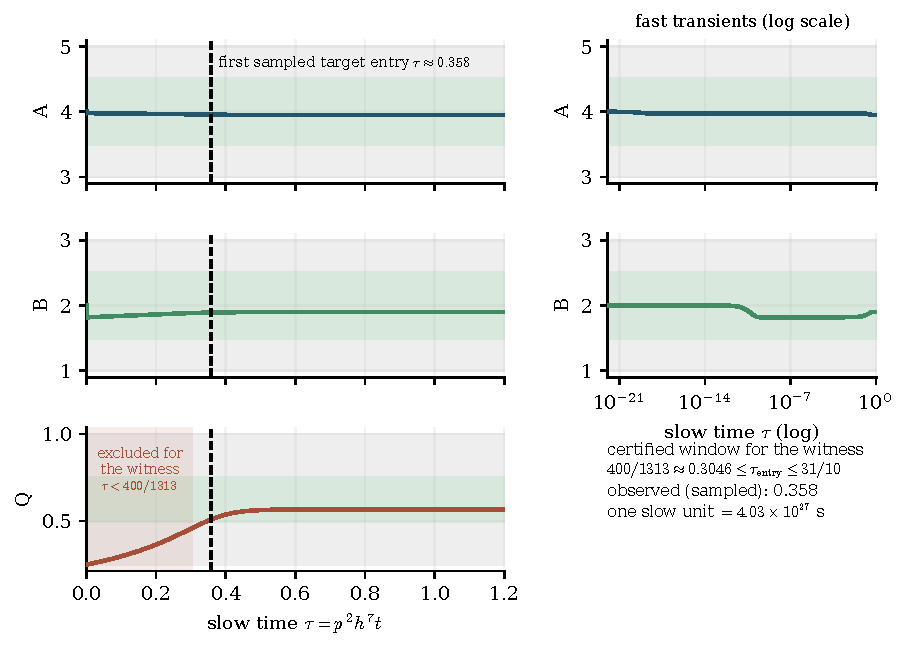
\includegraphics[width=\linewidth]{recovery_trajectory}
\caption{Numerical illustration of the complete system~\eqref{eq:currents} at $h=1/600$, $u=1/20$, nominal prefactors, from the witness~\eqref{eq:witness}, plotted against the exact slow time $\tau=p^2h^7t$ (left) and on a logarithmic time axis for the fast coordinates (right). Grey bands are the outer intervals of $\calO$, green bands the target intervals of $\calI$. The dashed vertical line marks the first sampled time at which all three coordinates lie in $\calI$, $\tau\approx0.358$; the shaded region $\tau<400/1313$ is excluded for the witness by Proposition~\ref{prop:witness}, and the certified deadline $\tau=31/10$ lies beyond the plotted window. One slow unit is $4.03\times10^{27}$ seconds in the calibration of Section~\ref{sec:examples}.}
\label{fig:trajectory}
\end{figure}

\subsection{Global inventory clocks for arbitrary seeds}
\label{sec:global-clocks}
Theorem~\ref{thm:coupled} assumes a prepared seed. The inventory identity, however, carries information on the whole positive orthant, because positivity alone gives
\begin{equation}\label{eq:orthant-bounds}
 z\le\tfrac12W,\qquad x\le\tfrac16W,\qquad y\le\tfrac15W\qquad\text{for every positive state}.
\end{equation}
Dropping the nonnegative term of the appropriate sign in $\dot W=-13J_3=-13a_3x^2y+13b_3ph^6z^2$ and inserting~\eqref{eq:orthant-bounds} gives the two-sided differential inequality
\begin{equation}\label{eq:W-inequality}
 -\tfrac{13}{180}\,a_3\,W^3\ \le\ \dot W\ \le\ \tfrac{13}{4}\,b_3ph^6\,W^2 ,
\end{equation}
valid along every positive solution at every time.

\begin{theorem}[Global inventory clocks]\label{thm:global-clocks}
Assume~\eqref{eq:parameters}. Every positive initial state has a global positive solution of~\eqref{eq:currents}, and every global positive solution satisfies, for all $T\ge0$,
\begin{align}
 T&\ \ge\ \frac{4}{13\,b_3\,ph^6}\Big(\frac1{W(0)}-\frac1{W(T)}\Big)
 &&\text{(restoration clock)},\label{eq:restoration-clock}\\
 T&\ \ge\ \frac{90}{13\,a_3}\Big(\frac1{W(T)^2}-\frac1{W(0)^2}\Big)
 &&\text{(depletion clock)}.\label{eq:depletion-clock}
\end{align}
In particular, any positive solution that raises its inventory from $W_0$ to $W_1>W_0$ needs time at least $\frac{4}{13b_3ph^6}(W_0^{-1}-W_1^{-1})$, and any solution that lowers it from $W_0$ to $W_1<W_0$ needs at least $\frac{90}{13a_3}(W_1^{-2}-W_0^{-2})$, whatever the shape coordinates $A,B$ do.
\end{theorem}

\begin{proof}
Global existence from every positive seed is the attributed global-solution theorem (Theorem~\ref{thm:imported}) applied to the weakly reversible network~\eqref{eq:reactions}. For~\eqref{eq:restoration-clock}, $f=1/W$ is $C^1$ with $f'=-\dot W/W^2\ge-\tfrac{13}{4}b_3ph^6$ by~\eqref{eq:W-inequality}; integrating, $f(0)-f(T)\le\tfrac{13}{4}b_3ph^6\,T$. For~\eqref{eq:depletion-clock}, $g=1/W^2$ has $g'=-2\dot W/W^3\le\tfrac{13}{90}a_3$, so $g(T)-g(0)\le\tfrac{13}{90}a_3T$. Neither bound uses monotonicity of $W$, so both hold at every time, not only at first passage.
\end{proof}

The restoration clock with $W(0)=\tfrac{ph}2$ and $W(T)\ge ph$ gives $T\ge\frac{4}{13b_3}\lambda^{-1}\ge\frac{400}{1313}\lambda^{-1}$: Proposition~\ref{prop:witness} is the special case of Theorem~\ref{thm:global-clocks} at the witness, and the prepared basin was never needed for the lower bound. The depletion clock quantifies the opposite transient: from a macroscopic seed such as $x=y=z=1$ ($W=13$), reaching the corridor inventory $W\le ph$ needs at least $\frac{90}{13a_3}\big((ph)^{-2}-13^{-2}\big)\approx6.9\,(ph)^{-2}$ time units at nominal $a_3$, which is $h^{5}$ times the restoration scale $\lambda^{-1}$: collapse of a surplus is governed by the forward reaction $2X+Y\to2Z$ and is at least $(ph)^{-2}$ slow, while rebuilding a deficit is $(p^2h^7)^{-1}$ slow. What the theorem does not give is an upper bound on the time for an arbitrary seed to enter the sharp corridor; see Section~\ref{sec:discussion}.

\section{Corollaries and the inventory mechanism}
\label{sec:corollaries}

\subsection{Common clocks}
\begin{corollary}[Exact common-clock transport]\label{cor:clock}
For autonomous mass action and $b>0$, $\tilde x$ is a global forward solution for rates $\tilde k$ if and only if $x(t)=\tilde x(bt)$ is a global forward solution for rates $k_e=b\tilde k_e$ from the same initial state. Phase-space paths, invariant sets and residence statements correspond exactly; all times are divided by $b$.
\end{corollary}

\begin{proof}
$f_{b\tilde k}=bf_{\tilde k}$, and the chain rule gives $\dot x(t)=b\dot{\tilde x}(bt)=bf_{\tilde k}(\tilde x(bt))=f_{b\tilde k}(x(t))$; the converse uses $b^{-1}$.
\end{proof}

This is why~\eqref{eq:general-bound} depends only on the spread $\Delta$: a common factor $\eps^{a_-}$ leaves concentration geometry unchanged and multiplies all times by $\eps^{-a_-}$. Different exponent assignments with the same spread can nevertheless have different sharp species scales, as the coupled network shows.

\subsection{A continuous reverse-exponent family}
Let $\tfrac12<\gamma<\tfrac72$ and set
\begin{equation}\label{eq:gamma-path}
 p=\eps^{1/2},\qquad h=\eps^{(2\gamma-1)/12},\qquad u=\eps^{(7-2\gamma)/12},
\end{equation}
so that $p=uh$, $p^2=\eps$ and $ph^6=\eps^\gamma$: the reverse rates on pairs $1,2,4$ are proportional to $\eps$ and pair $3$ has reverse exponent $\gamma$.

\begin{corollary}[Certified exponent family]\label{cor:gamma}
Define
\begin{equation}\label{eq:improved-cutoff}
 \eps_{\max}(\gamma)=\min\big\{600^{-12/(2\gamma-1)},\ 20^{-12/(7-2\gamma)}\big\}.
\end{equation}
For $0<\eps\le\eps_{\max}(\gamma)$ and all admitted prefactors, Theorem~\ref{thm:coupled} applies to~\eqref{eq:gamma-path}. Along every prepared trajectory,
\begin{equation}\label{eq:gamma-orders}
 x\asymp\eps^{(2\gamma+1)/4},\qquad y\asymp\eps^{(\gamma+1)/3},\qquad z\asymp\eps^{(2\gamma+5)/12},
\end{equation}
with the explicit constants of~\eqref{eq:sharp-bounds}; every prepared start recovers by $\tfrac{31}{10}\eps^{-(14\gamma+5)/12}$ and the witness needs at least $\tfrac{400}{1313}\eps^{-(14\gamma+5)/12}$.
\end{corollary}

\begin{proof}
$h\le\tfrac1{600}$ and $u\le\tfrac1{20}$ are exactly the two real-power inequalities in~\eqref{eq:improved-cutoff}, and $ph^3=\eps^{(2\gamma+1)/4}$, $ph^2=\eps^{(\gamma+1)/3}$, $ph=\eps^{(2\gamma+5)/12}$, $p^2h^7=\eps^{(14\gamma+5)/12}$ by exponent arithmetic. Substitute into Theorem~\ref{thm:coupled}.
\end{proof}

The earlier symmetric restriction $h,u\le10^{-3}$ corresponds to the cutoff
\begin{equation}\label{eq:original-cutoff}
 \eps\le10^{-36/\min\{2\gamma-1,\,7-2\gamma\}};
\end{equation}
at $\gamma=1$ it gives $10^{-36}$, while~\eqref{eq:improved-cutoff} gives $600^{-12}\approx4.59\times10^{-34}$. At $\gamma=2$ the concentration exponents are $\tfrac54,1,\tfrac34$ and the recovery exponent $\tfrac{11}4$. The endpoints $\gamma=\tfrac12$ and $\tfrac72$ are not covered: there one of $h,u$ stops tending to zero. Figure~\ref{fig:exponents} displays the exponent laws and the cutoffs.

\begin{figure}[tb]
\centering
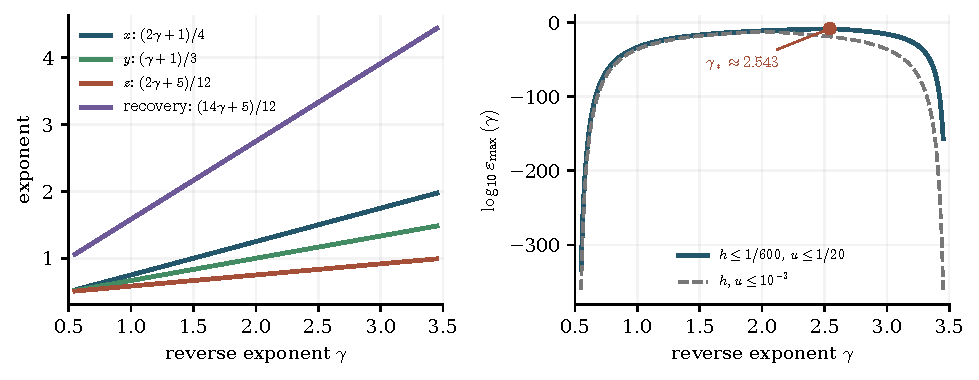
\includegraphics[width=\linewidth]{exponent_family}
\caption{Left: exponent laws~\eqref{eq:gamma-orders} and the recovery exponent along the family~\eqref{eq:gamma-path}. Right: the certified cutoff $\log_{10}\eps_{\max}(\gamma)$ for the current rectangle (solid) and for the original symmetric restriction (dashed). The marked point is the corner $\gamma_*$ of Proposition~\ref{prop:corner}, where the two branches of~\eqref{eq:improved-cutoff} balance and $\eps_{\max}$ attains its largest value $1/144{,}000{,}000$.}
\label{fig:exponents}
\end{figure}

\begin{proposition}[Best corner of the certificate]\label{prop:corner}
Over the rectangle~\eqref{eq:parameters}, $p=uh\le\tfrac1{12000}$, so the baseline reverse parameter satisfies $\eps=p^2\le\tfrac1{144{,}000{,}000}\approx6.94\times10^{-9}$. The family~\eqref{eq:gamma-path} reaches this corner exactly when
\begin{equation}\label{eq:gamma-star}
 \gamma_*=\frac12+\frac{3\ln600}{\ln12000}\approx2.5432 ,
\end{equation}
which maximises $\eps_{\max}(\gamma)$. For fixed $p\le\tfrac1{12000}$ the admissible $h$ range is $[20p,\tfrac1{600}]$, and $\lambda=p^2h^7$ is increasing in $h$ and in $p$, so the fastest certified recovery scale over the whole rectangle is attained at $h=\tfrac1{600}$, $u=\tfrac1{20}$:
\begin{equation}\label{eq:corner-scale}
 \lambda^{-1}=12000^2\cdot600^7=4.0310784\times10^{27}.
\end{equation}
\end{proposition}

\begin{proof}
The two branches of~\eqref{eq:improved-cutoff} are respectively increasing and decreasing in $\gamma$ and balance when $(7-2\gamma)\ln600=(2\gamma-1)\ln20$, i.e.\ at~\eqref{eq:gamma-star}; substituting $h=\tfrac1{600}$, $p=\tfrac1{12000}$ into~\eqref{eq:gamma-path} gives the same value. The remaining statements are monotonicity of $p^2h^7$ in each variable.
\end{proof}

Figure~\ref{fig:rectangle} shows $\log_{10}\lambda^{-1}$ over the rectangle together with two family paths. The corner is where the certificate is least pessimistic; it is not an optimised physical design, and enlarging the rectangle would require a new certificate (Section~\ref{sec:discussion}).

\begin{figure}[tb]
\centering
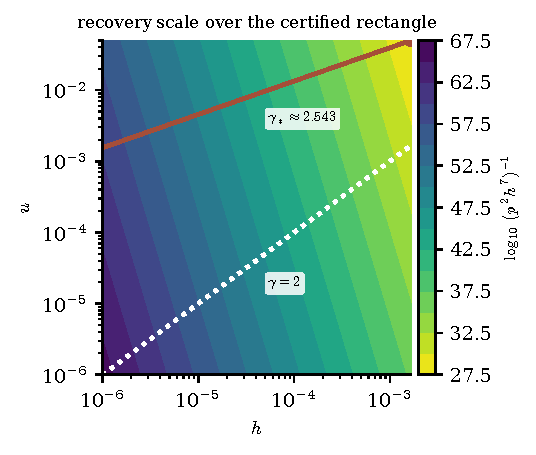
\includegraphics[width=.55\linewidth]{parameter_rectangle}
\caption{The certified recovery scale $\log_{10}(p^2h^7)^{-1}$ over the admitted rectangle (logarithmic axes). Dotted: the family path $\gamma=2$. Solid: the path $\gamma_*\approx2.543$, which passes through the corner $(h,u)=(1/600,1/20)$ (dot), the point of fastest certified recovery.}
\label{fig:rectangle}
\end{figure}

\subsection{Scale identities and necessary reaction extent}
\begin{corollary}[Preparation--recovery trade-off]\label{cor:tradeoff}
With the preparation scales $s_x=ph^3$, $s_y=ph^2$, $s_z=ph$,
\begin{equation}\label{eq:tradeoff}
 s_y^2=s_xs_z,\qquad \lambda^{-1}=\frac{s_y}{s_x^3}=\frac{s_z^3}{s_y^5}.
\end{equation}
Hence the witness lower bound and the universal prepared deadline are $\tfrac{400}{1313}s_y/s_x^3$ and $\tfrac{31}{10}s_y/s_x^3$.
\end{corollary}

\begin{proof}
Substitute and cancel positive powers of $p$ and $h$.
\end{proof}

These are identities among dimensionless preparation scales, not formulas in arbitrary measured concentrations; they explain why extreme separation of concentration scales in this family is accompanied by slow recovery.

\begin{corollary}[Necessary cumulative reverse extent]\label{cor:extent}
For any solution from~\eqref{eq:witness} and any $T\ge0$ at which it is in the target,
\begin{equation}\label{eq:extent}
 -\int_0^TJ_3(t)\dd t=\frac{W(T)-W(0)}{13}\ \ge\ \frac{ph}{26},\qquad \int_0^Tb_3ph^6z(t)^2\dd t\ \ge\ \frac{ph}{26}.
\end{equation}
\end{corollary}

\begin{proof}
Integrate~\eqref{eq:neutral}; $W=2phQ$ rises from $\tfrac{ph}2$ to at least $ph$. Since $-J_3=b_3ph^6z^2-a_3x^2y\le b_3ph^6z^2$, the second bound follows.
\end{proof}

\subsection{A general inventory-bottleneck principle}
\label{sec:bottleneck}
The witness argument is an instance of a general principle that uses stoichiometry and kinetics rather than the reaction graph alone. Write a mass-action system as $\dot x=\sum_e\nu_ev_e(x)$ with $v_e\ge0$, each direction of a reversible pair counted separately.

\begin{proposition}[Inventory bottleneck, constant capacity]\label{prop:bottleneck}
Partition the reactions into a fast set $F$ and a remainder $R$, and let $\ell\in\R^d$ satisfy $\ell\cdot\nu_e=0$ for all $e\in F$. Put $U=\ell\cdot x$. Suppose that, up to the target time $T$, the trajectory stays in a region $\calD$ on which
\[
 \sum_{e\in R}(\ell\cdot\nu_e)_+\,v_e(x)\le M .
\]
If reaching the target requires $U(T)\ge U(0)+\Delta U$ with $\Delta U>0$, then $T\ge\Delta U/M$ when $M>0$, and the target is unreachable along such a trajectory when $M=0$.
\end{proposition}

\begin{proof}
$\dot U=\sum_{e\in R}(\ell\cdot\nu_e)v_e\le\sum_{e\in R}(\ell\cdot\nu_e)_+v_e\le M$ on $\calD$; integrate. No monotonicity of $U$ is needed.
\end{proof}

\begin{proposition}[Inventory bottleneck, state-dependent capacity]\label{prop:bottleneck-state}
In the setting of Proposition~\ref{prop:bottleneck} suppose instead that $\dot U\le g(U)$ on $\calD$ for a continuous $g>0$ on an interval containing $[U(0),U_{\rm target}]$ and all values taken by $U$ before $T$. Then
\begin{equation}\label{eq:state-capacity}
 T\ \ge\ \int_{U(0)}^{U_{\rm target}}\frac{\dd s}{g(s)} .
\end{equation}
\end{proposition}

\begin{proof}
Let $\Phi'=1/g$; then $(\Phi\circ U)'=\dot U/g(U)\le1$, so $\Phi(U(T))-\Phi(U(0))\le T$, and $\Phi$ is increasing. The selected formal statement assumes an open containing interval and the derivative bound on the closed time interval $[0,T]$. It covers the positive-inventory applications below; the more general interval formulation here retains its conventional proof.
\end{proof}

\begin{corollary}[Explicit $\eps$-scaling]\label{cor:scaling}
In the setting of Proposition~\ref{prop:bottleneck}, suppose every reaction $e\in R$ with $\ell\cdot\nu_e>0$ has rate $k_e=\bar k_e\eps^{a_e}$ with $a_e\ge a$ and $\bar k_e\le\kappa_+$, and that $x^{y_e}\le m_e$ on $\calD$. Then any target requiring $U$ to rise by $\Delta U>0$ satisfies
\begin{equation}\label{eq:scaling}
 T\ \ge\ \frac{\Delta U}{\kappa_+\sum_{e\in R,\ \ell\cdot\nu_e>0}(\ell\cdot\nu_e)\,m_e}\ \eps^{-a}\ =\ \Omega(\eps^{-a}),
\end{equation}
uniformly over the admitted prefactors. In the general setting of Theorem~\ref{thm:general}, after the entry time the trajectory lies in the box~\eqref{eq:general-bound}, so $m_e=(\alpha^{-1/2}\eps^{-\Delta/(2H)})^{|y_e|}$ is admissible and~\eqref{eq:scaling} holds from that time on.
\end{corollary}

\begin{proof}
$\dot U\le\sum(\ell\cdot\nu_e)_+k_ex^{y_e}\le\eps^a\kappa_+\sum(\ell\cdot\nu_e)_+m_e=:C\eps^a$ on $\calD$, and Proposition~\ref{prop:bottleneck} with $M=C\eps^a$ gives $T\ge(\Delta U/C)\eps^{-a}$.
\end{proof}

This is the universal form of the slow-channel obstruction: it needs only stoichiometry (a left null vector of the fast reaction vectors), the slow rate scalings and a region bound, never the graph alone and never the constant $H$. It is one-sided; a matching upper bound requires network-specific progress estimates, which is what Theorem~\ref{thm:coupled} supplies for~\eqref{eq:reactions}. For the coupled network take $\ell=(6,5,2)$, $F$ the six directed reactions of pairs $1,2,4$, and $R$ the two directions of pair $3$. The only positive contribution to $\dot W$ is $13\,b_3ph^6z^2$, and on the preimage of $\calO$ we have $z=phQC\le phQ=W/2$, so $\dot W\le g(W):=\tfrac{13}{4}b_3ph^6W^2$. For the witness $W$ must rise from $\tfrac{ph}{2}$ to $ph$, and~\eqref{eq:state-capacity} gives
\[
 T\ \ge\ \frac{4}{13\,b_3\,ph^6}\Big(\frac{2}{ph}-\frac1{ph}\Big)=\frac{4}{13\,b_3}\,\lambda^{-1}\ \ge\ \frac{400}{1313}\,\lambda^{-1},
\]
which is Proposition~\ref{prop:witness} and, since~\eqref{eq:orthant-bounds} needs no basin, Theorem~\ref{thm:global-clocks}: the reciprocal comparison \emph{is} the state-dependent capacity bound for $g(W)\propto W^2$. The constant-capacity version with $z\le ph$ gives the weaker $T\ge\lambda^{-1}/(26\cdot\tfrac{101}{100})$, and Corollary~\ref{cor:scaling} with $a=\gamma$ along the family~\eqref{eq:gamma-path} gives the recovery exponent up to the region-dependent prefactor. Conversely, a capacity bound alone never yields a matching upper bound; the deadline requires independent forward progress ($R_Q\ge\tfrac1{10}$ on the slab) and invariance of the comparison region.

Fast-subsystem conservation laws as slow variables have an established literature; see~\cite{Desoeuvres2024} for approximate conservation laws and reduction, and~\cite{Fenichel1979} for the geometric theory. The propositions above are elementary; their value is that they turn such an inventory into an explicit, regionally justified lower bound on recovery time. The productive search pattern for related mechanisms is: candidate fast subnetwork $\to$ exact left null vector $\ell$ $\to$ regional bound on the increasing slow fluxes $\to$ lower time bound $\to$ a separate progress mechanism for an upper bound. The reaction graph alone does not determine $\ell$, the flux bound or a useful region.

\section{Stochastic remarks}
\label{sec:stochastic}
Consider the standard stochastic mass-action model of~\eqref{eq:reactions}, a continuous-time Markov chain on molecule counts $n=(n_X,n_Y,n_Z)\in\N^3$ with combinatorial propensities~\cite{Kurtz1972,Gillespie1977,AndersonKurtz2015}, in which every one of the eight directed reactions has a positive rate constant.

\begin{proposition}[No jump into an absorbing state]\label{prop:absorbing}
\begin{enumerate}[label=(\alph*)]
\item For any reversible network with all rate constants positive, no reaction event can lead from a state in which some reaction is enabled to a state in which no reaction is enabled.
\item For~\eqref{eq:reactions} the absorbing count states are exactly $(0,0,0)$, $(0,1,0)$, $(0,0,1)$ and $(0,1,1)$, and none of them is reachable from any other state.
\end{enumerate}
\end{proposition}

\begin{proof}
(a) A jump consuming the complex $y$ and producing $y'$ leaves a state containing at least $y'$ molecules of the product complex, so the reverse reaction $y'\to y$, which has positive rate, is enabled at the destination. (b) $n_X\ge1$ enables $X\to3Z$; $n_Y\ge2$ enables $2Y\to X+2Z$; $n_Z\ge2$ enables $2Z\to2X+Y$. If none holds then $n_X=0$, $n_Y\le1$, $n_Z\le1$, and inspection shows that none of the eight reactions is enabled. Unreachability is (a).
\end{proof}

Consequently the inventory bottleneck must not be interpreted as a mechanism of high-probability absorbing extinction for the literal reversible network. Individual species counts can reach zero and return (for instance $n_X=0$ is left by $3Z\to X$); species absence, loss of a function threshold and absorption are different events and should be measured separately in simulations. Proposition~\ref{prop:absorbing} says nothing about nonexplosion, positive recurrence or stationary distributions; for weakly reversible networks with a single linkage class such questions are treated in~\cite{AndersonCappellettiKim2019}, but this network has four linkage classes and those results do not apply without further hypotheses.

The deterministic identity~\eqref{eq:neutral} has an exact discrete counterpart. Let $N_3^{+}(t)$ and $N_3^{-}(t)$ count the forward and reverse events of pair $3$ and put $W_n=6n_X+5n_Y+2n_Z$. Before any explosion,
\begin{equation}\label{eq:discrete-inventory}
 W_n(t)=W_n(0)+13\big(N_3^-(t)-N_3^+(t)\big),
\end{equation}
so $W_n\bmod13$ is invariant, and a target requiring $W_n$ to rise by at least $L$ requires at least $m=\lceil L/13\rceil$ reverse events of pair $3$.

The reverse propensity of pair $3$ is $\lambda_3^-(n)=\kappa\,n_Z(n_Z-1)$ with $\kappa=b_3ph^6/(VN_{\!A})$ in the units of Section~\ref{sec:examples}, and $2n_Z\le W_n$ for every count state. Hence $\lambda_3^-\le\tfrac{\kappa}{4}W_n^2$ everywhere, which is the discrete form of~\eqref{eq:W-inequality}. This turns the inventory bottleneck into a pathwise statement with no localisation.

\begin{proposition}[Pure-birth comparison]\label{prop:birth}
Let $W_0=W_n(0)$ and let $T$ be any random time at which $W_n(T)\ge W_0+13m$ for an integer $m\ge1$ (with $T=\infty$ if this never happens before explosion). Put $g_k=\tfrac{\kappa}{4}(W_0+13k)^2$. Then there are i.i.d.\ unit exponential random variables $E_0,\dots,E_{m-1}$ with
\begin{equation}\label{eq:birth-pathwise}
 T\ \ge\ \sum_{k=0}^{m-1}\frac{E_k}{g_k}\qquad\text{pathwise}.
\end{equation}
Consequently
\begin{equation}\label{eq:birth-moments}
 \mathbb E[T]\ \ge\ \sum_{k=0}^{m-1}\frac1{g_k}\ \ge\ \frac{4}{13\kappa}\Big(\frac1{W_0}-\frac1{W_0+13m}\Big),\qquad
 \Pr\{T\le t\}\ \le\ e^{\theta t}\prod_{k=0}^{m-1}\Big(1+\frac\theta{g_k}\Big)^{-1}\quad(\theta>0),
\end{equation}
and the lower bound in~\eqref{eq:birth-pathwise} has variance $\sum_kg_k^{-2}$.
\end{proposition}

\begin{proof}
By the random time-change representation~\cite{Kurtz1972,AndersonKurtz2015}, $N_3^-(t)=Y\big(\int_0^t\lambda_3^-(n(s))\dd s\big)$ for a unit-rate Poisson process $Y$, up to explosion. Let $\sigma_k$ be the time of the $k$-th reverse pair-$3$ event and $E_k$ the $k$-th interarrival time of $Y$, so the $E_k$ are i.i.d.\ unit exponentials. Forward pair-$3$ events lower $W_n$ and all other events preserve it, so $W_n(s)\le W_0+13N_3^-(s)$ by~\eqref{eq:discrete-inventory}; on $(\sigma_k,\sigma_{k+1}]$ we have $N_3^-=k$ and therefore $\lambda_3^-\le\tfrac\kappa4(W_0+13k)^2=g_k$. Hence $E_k=\int_{\sigma_k}^{\sigma_{k+1}}\lambda_3^-\le g_k(\sigma_{k+1}-\sigma_k)$. Reaching $W_n\ge W_0+13m$ requires $N_3^-\ge m$, so $T\ge\sigma_m=\sum_{k<m}(\sigma_{k+1}-\sigma_k)\ge\sum_{k<m}E_k/g_k$. The expectation, the integral comparison $\sum_{k<m}(W_0+13k)^{-2}\ge\int_0^m(W_0+13s)^{-2}\dd s$, the variance and the Chernoff bound $\Pr\{S\le t\}\le e^{\theta t}\mathbb E e^{-\theta S}$ follow from independence.
\end{proof}

Writing $W_n=WVN_{\!A}$ and $\kappa=b_3ph^6/(VN_{\!A})$, the mean bound in~\eqref{eq:birth-moments} is exactly the deterministic restoration clock~\eqref{eq:restoration-clock}, up to the discreteness correction $W_0+13m$ versus $W_1$: the deterministic clock is the expectation of a pathwise stochastic lower bound. At the corner of Section~\ref{sec:examples} ($V=1\,\mathrm L$), $W_0=4.18\times10^{16}$ counts, $m=3.2\times10^{15}$, and the bound has mean $1.228\times10^{27}\,\mathrm s$ with relative standard deviation $1.9\times10^{-8}$; the stochastic recovery time is at least this, essentially deterministically. At the reference endpoint $\eps=10^{-36}$, where the deterministic $X$ concentration corresponds to $0.003$ molecules, the inventory sits almost entirely in $Z$: $W_0\approx301$ counts, $m=24$, mean bound $3.2\times10^{56}\,\mathrm s$ with relative standard deviation $0.22$. The bottleneck therefore survives the breakdown of the deterministic description; what changes at low counts is the width of the distribution, not the order of the delay. No finite localisation, nonexplosion assumption or bound on other species is needed, because the comparison uses only the inventory itself.

For completeness, a localised Poisson bound also holds: if the reverse propensity is at most $\Lambda$ on a finite set $\calD$ of count states, then $\Pr\{T_{\rm target}\le t,\ T_{\rm target}\le\tau_{\rm exit}\}\le\Pr\{\mathrm{Poisson}(\Lambda t)\ge m\}$. It is weaker than Proposition~\ref{prop:birth}: at the corner, bounding $n_Z$ by its outer-box maximum gives $m/\Lambda\approx1.5\times10^{26}\,\mathrm s$, a factor eight below the birth-chain mean, because it ignores that the propensity is smallest exactly when the deficit is largest.

\section{Dimensional calibration and operational limitations}
\label{sec:examples}
Fix a concentration unit $C_0$, a time unit $\tau_0$ and a volume $V$, independently of the parameters. If $\hat k$ is a dimensionless rate constant for a source of molecularity $|y|$, then
\begin{equation}\label{eq:dimensional}
 k_{\rm dim}=\frac{\hat kC_0^{1-|y|}}{\tau_0},\qquad c_i=C_0x_i,\qquad t_{\rm dim}=\tau_0t,\qquad N_i=c_iVN_{\!A},
\end{equation}
with $N_{\!A}=6.02214076\times10^{23}\,\mathrm{mol^{-1}}$ exactly~\cite{BIPM2019}. All forward sources in~\eqref{eq:reactions} are cubic; the reverse sources of pairs $1$--$3$ are quadratic and that of pair $4$ is linear. Take $C_0=1\,\mathrm{mol\,L^{-1}}$, $\tau_0=1\,\mathrm s$, $V=1\,\mathrm L$ and the corner $h=\tfrac1{600}$, $u=\tfrac1{20}$ ($p=\tfrac1{12000}$) with nominal prefactors. The forward constants are $1,1,1,4\ \mathrm{L^2mol^{-2}s^{-1}}$; the reverse constants are $6.944\times10^{-9}\ \mathrm{L\,mol^{-1}s^{-1}}$ for pairs $1$ and $2$, $1.786\times10^{-21}\ \mathrm{L\,mol^{-1}s^{-1}}$ for pair $3$ and $6.944\times10^{-9}\ \mathrm{s^{-1}}$ for pair $4$. The certified all-time bounds, rounded outward, are
\begin{center}
\begin{tabular}{lrrr}
\toprule
species & lower bound (mol/L) & upper bound (mol/L) & upper count in $1\,\mathrm L$\\
\midrule
$X$ & $1.8084\times10^{-14}$ & $1.9291\times10^{-12}$ & $1.1617\times10^{12}$\\
$Y$ & $1.4467\times10^{-11}$ & $6.9445\times10^{-10}$ & $4.1821\times10^{14}$\\
$Z$ & $1.7361\times10^{-8}$ & $1.3889\times10^{-7}$ & $8.3641\times10^{16}$\\
\bottomrule
\end{tabular}
\end{center}
and the certified recovery window is
\[
 1.2281\times10^{27}\,\mathrm s\ \le\ T_{\rm witness},\qquad T_{\rm all}\ \le\ 1.2497\times10^{28}\,\mathrm s .
\]
Copy numbers are macroscopic, yet the certified recovery time exceeds the age of the universe by nine orders of magnitude. No small time unit has been chosen to hide this.

Other admissible points have the opposite limitation. On the reference path $\gamma=1$ at the original endpoint $\eps=10^{-36}$, the upper bound for $X$ is $5\times10^{-27}\,\mathrm{mol/L}$, fewer than $0.004$ expected molecules in one litre, with $3.05\times10^{56}\,\mathrm s\le T_{\rm witness}$ and $T_{\rm all}\le3.1\times10^{57}\,\mathrm s$; at the improved endpoint $\eps=600^{-12}$ the $X$ upper count is still below $0.30$, with $1.86\times10^{52}\,\mathrm s\le T_{\rm witness}$ and $T_{\rm all}\le1.89\times10^{53}\,\mathrm s$. These are expected-count readings of continuous concentrations, not claims about fractional molecules; a deterministic description is not justified at such counts.

There is also a thermodynamic distinction. With $r_i$ the forward-to-reverse ratio of pair $i$ on the reference path, the rate ratio around the independent cycle formed by pairs $1$, $2$ and $4$ is
\begin{equation}\label{eq:cycle-ratio}
 \frac{r_1r_2}{r_4}=\frac1{4\eps},
\end{equation}
whose logarithm is about $81.5$ at $\eps=10^{-36}$ and $17.4$ at the corner. Graph reversibility therefore does not imply equilibrium thermodynamic reversibility; reading such a cycle logarithm as an affinity or chemical work~\cite{Schnakenberg1976} requires a thermodynamically specified reservoir realisation that this three-species effective model does not supply. For practitioners the model-specific conclusion is: adding tiny reverse reactions can restore mathematical permanence while the certified concentrations or recovery times remain operationally unacceptable. This is a diagnostic pattern (identify nearly conserved inventories, bound their replenishment capacity, compare with the operating horizon, check copy numbers), not a universal obstruction to useful reversible chemistry.

\section{Formal verification and reproducibility}
\label{sec:formal}

\paragraph{Environment and root.}
The deterministic containment, prepared recovery, lower witness, global inventory clocks, continuous exponent family, time transport, preparation identities, reverse extent, and abstract constant-capacity results have saved strict checks in Lean~4 (native toolchain \lean{v4.30.0}) against a frozen Mathlib snapshot~\cite{Lean4,Mathlib2020}. The conventional items are identified in Table~\ref{tab:evidence}. The governing declaration is the theorem \lean{Publication.Main} in the namespace \lean{ReverseRateLimits}: its hypotheses are a finite weakly reversible network, the parameter data~\eqref{eq:parameters} as a structure with positivity and interval fields, and a positive prepared initial state; its conclusion is the conjunction of Theorem~\ref{thm:general}, Theorem~\ref{thm:coupled} (with the constants $31/10$ and $400/1313$), Theorem~\ref{thm:global-clocks} (existence from every positive seed and both clocks for every global positive solution), Corollary~\ref{cor:extent}, Corollary~\ref{cor:clock}, Corollary~\ref{cor:tradeoff}, Corollary~\ref{cor:gamma} with both cutoffs, and the absence of a linear conservation law. Definitions of trajectories contain only the three literal derivative equations and positivity; region membership, invariance, deadlines and witnesses are proved, never assumed. Compilation treats warnings as errors and probes the exported declaration interfaces; the only axioms reported are \lean{propext}, \lean{Classical.choice} and \lean{Quot.sound}.

\paragraph{Submission checks.}
The standalone submission uses Lean~4.35.0-rc2 with its pinned Mathlib manifest. Eighteen selected declarations expose the general containment and global clocks independently of the bundled prepared-state premises. They include the rates-preserving family constructor, an admitted parameter instance, and the open-range form of Proposition~\ref{prop:bottleneck-state}. Strict compilation and standard-axiom probes, comparison with an independent Mathlib-only statement, and all six configured kernel checks pass for the recorded source hashes. The checked kernels are Lean paranoid, lean4lean, nanoda, con-leche, con-ron and Lean default. Portable evidence summaries and the exact selected claim map accompany the sources.

\paragraph{Attributed input.}
The affine geometry (Theorem~\ref{thm:imported}) is imported from the pinned revision \lean{adc7f1241b42e322a6451854ab7e4b4c146bf78a} of~\cite{OpenAI2026Formal} through three declarations:
\begin{itemize}
\item \lean{Affine.exists\_fullCertificate} (existence of the label set for a prescribed tolerance),
\item \lean{FullCertificate.uniform\_activity} (the uniform activity property), and
\item \lean{global\_bounded\_persistent\_solution} (global positive solutions with compact bounds).
\end{itemize}
The native sources were compiled after recorded compatibility adaptations to their frozen Mathlib snapshot. The submission port preserves module names and records the corresponding changes separately in its migration provenance.

\paragraph{Declaration map.}
Table~\ref{tab:declarations} maps the claims of this paper to the Lean declarations that prove them, and Table~\ref{tab:evidence} summarises the evidence level of every item.

\begin{table}[htb]
\centering\small
\caption{Declaration map (default namespace \lean{ReverseRateLimits}).}
\label{tab:declarations}
\begin{tabular}{>{\raggedright\arraybackslash}p{.33\linewidth}>{\raggedright\arraybackslash}p{.60\linewidth}}
\toprule
claim & Lean declaration\\
\midrule
Lemma~\ref{lem:drift} (cut drift) & \lean{QuantitativeDrift.massAction\_quantitative\_drift}\\
Lemma~\ref{lem:entry} (one-scale entry) & \lean{ScaleEntry.ScalePlateau.entry}\\
dyadic descent & \lean{ScaleChain.dyadic\_plateau\_descent}\\
classwise absorption & \lean{ClasswiseAbsorption.classwise\_absorption}\\
Theorem~\ref{thm:general} & \lean{general\_quantitative\_root}\\
\eqref{eq:neutral}, transformed field & \lean{CoupledSource.neutral\_pool}, \lean{CoupledSource.transformed\_source}\\
Lemma~\ref{lem:corridor} (18 inclusions) & \lean{SourceBounds.outer\_*}, \lean{SourceBounds.inner\_*}, \lean{SourceBounds.entry\_*}; checker \lean{IntervalCertificate.Expr.sound}\\
Proposition~\ref{prop:invariance} & \lean{CorridorDynamics.outer\_invariant}, \lean{SourceExistence.exists\_literal\_trajectory}, \lean{PhysicalBounds.all\_time\_coordinate\_bounds}\\
Lemma~\ref{lem:slab} & \lean{lower\_entry}, \lean{upper\_entry}\\
Proposition~\ref{prop:deadline} & \lean{CorridorDynamics.entry\_A}, \lean{entry\_B}, \lean{SharpRecovery.entry\_Q\_sharp}, \lean{SharpRecovery.deadline\_sharp}\\
Proposition~\ref{prop:witness} & \lean{SharpRecovery.witness\_time\_lower\_sharp}, \lean{SharpRecovery.witness\_sharp}\\
Theorem~\ref{thm:coupled} & \lean{SharpRecovery.prepared\_recovery\_sharp}, \lean{SharpRecovery.witness\_sharp}\\
\eqref{eq:W-inequality} & \lean{GlobalInventory.deriv\_inventory\_upper}, \lean{GlobalInventory.deriv\_inventory\_lower}\\
Theorem~\ref{thm:global-clocks} & \lean{GlobalInventory.restoration\_clock}, \lean{GlobalInventory.depletion\_clock}, \lean{GlobalInventory.global\_inventory\_clocks}; witness as special case \lean{GlobalInventory.witness\_from\_global\_clock}\\
Corollary~\ref{cor:clock} & \lean{CommonClock.rescale\_iff}\\
Corollary~\ref{cor:gamma} & \lean{SharpRecovery.family\_root\_sharp}, \lean{ExponentFamily.improved\_cutoff\_bounds}, \lean{ExponentFamily.original\_cutoff\_bounds}\\
Corollary~\ref{cor:tradeoff} & \lean{RecoveryCorollaries.scale\_tradeoff}\\
Corollary~\ref{cor:extent} & \lean{ReactionExtent.integral\_identity}, \lean{ReactionExtent.restoration\_extent}\\
Proposition~\ref{prop:bottleneck} & \lean{SharpRecovery.inventory\_bottleneck}, \lean{SharpRecovery.inventory\_unreachable}\\
Proposition~\ref{prop:bottleneck-state} (open interval form) & \lean{QuantitativeRegistry.state\_capacity\_clock}\\
Corollary~\ref{cor:scaling} (abstract form $\dot U\le C\eps^a$) & \lean{GlobalInventory.inventory\_bottleneck\_scaling}\\
no conservation law & \lean{RecoveryCorollaries.no\_linear\_inventory}\\
\bottomrule
\end{tabular}
\end{table}

\begin{table}[htb]
\centering\small
\caption{Evidence levels.}
\label{tab:evidence}
\begin{tabular}{>{\raggedright\arraybackslash}p{.52\linewidth}>{\raggedright\arraybackslash}p{.42\linewidth}}
\toprule
item & status\\
\midrule
Theorems~\ref{thm:general}, \ref{thm:coupled}, \ref{thm:global-clocks}; Lemmas~\ref{lem:drift}--\ref{lem:slab}; Corollaries~\ref{cor:clock}--\ref{cor:extent}; Proposition~\ref{prop:bottleneck}; Corollary~\ref{cor:scaling} in the abstract form $\dot U\le C\eps^a$ & formal (Lean, standard axioms)\\
Proposition~\ref{prop:bottleneck-state}, open containing interval & formal (Lean, standard axioms)\\
Theorem~\ref{thm:imported} & attributed, compiled from pinned source\\
Proposition~\ref{prop:bottleneck-state} beyond its open interval formal scope, Propositions~\ref{prop:absorbing}--\ref{prop:birth}, Proposition~\ref{prop:corner}, the flux bookkeeping in Corollary~\ref{cor:scaling} & conventional proofs in this paper; corner and birth-chain values by exact rational arithmetic\\
Figure~\ref{fig:trajectory}, observed entry $\tau\approx0.358$ & numerical illustration only\\
whole-class capture with an upper bound, optimal constants, limit of the scaled entry time, effective $H$, stochastic upper bounds & open (Section~\ref{sec:discussion})\\
\bottomrule
\end{tabular}
\end{table}

\paragraph{Numerical protocol.}
The trajectory of Figure~\ref{fig:trajectory} was computed with \textsc{SciPy}'s Radau integrator on~\eqref{eq:three-fields} with the exact symbolic Jacobian, relative tolerance $2\times10^{-6}$, absolute tolerance $2\times10^{-8}$, a first slow step of $10^{-22}$ and a fixed output grid; the run used $712$ function and $15$ Jacobian evaluations. Positivity, reconstruction of $(x,y,z)$, the inventory identity and target membership were checked on the output. The reported entry time is the first grid point inside $\calI$; it is a sampled observation, not a certified hitting time. The source package contains the complete proof dependency closure, certificate data, saved trajectory data, figure producers, and separately labelled native and submission-toolchain verification records. The standalone build instructions use the submitted paths.

\section{Discussion and open problems}
\label{sec:discussion}
Weak reversibility protects against concentration loss quantitatively as rates degenerate, but concentration geometry, preparation and recovery obey different laws. The general bound is governed by the exponent spread and an existence constant $H$. In the coupled network the preparation scales obey exact algebraic relations, the slow reverse reaction must supply a definite cumulative inventory restoration, and the state-dependent capacity bound reproduces the certified witness constant exactly. These facts explain the recovery exponent $(14\gamma+5)/12$ without any convergence or equilibrium argument.

\begin{enumerate}[label=(O\arabic*)]
\item \emph{Whole-class capture.} Theorem~\ref{thm:coupled} is restricted to the prepared basin. Theorem~\ref{thm:global-clocks} removes the basin hypothesis from the \emph{lower} bounds: from any positive seed, restoring a deficit costs at least the restoration clock and shedding a surplus at least the depletion clock. The general theorem absorbs every positive seed into a reciprocal box, but neither result gives a seed-independent deadline for entering the sharp corridor. A capture theorem would need to control $A$ and $B$ before corridor entry; the inventory identity alone does not, since $\dot Q$ depends on $A^2BQ^6$ and the identity gives no bound on $A,B$.
\item \emph{Limiting scaled entry time.} Matching powers do not give a limit for $\lambda T_{\rm entry}$ as $h,u\to0$. A candidate reduced slow equation after fast-layer control, with a quantified residual, is the natural next deliverable.
\item \emph{Optimal constants.} The window $[0.3046,3.1]$ is certified, not optimal; the sampled trajectory suggests the true worst case is near the lower end. Subdividing the entry slabs would sharpen the $A$ and $B$ phases, which are negligible here, and the $Q$ phase through a better bound on $R_Q$ along the actual corridor.
\item \emph{Larger rectangles.} At $h\le\tfrac1{500}$ with $u\le10^{-3}$ only the sufficient lower $A$ entry margin falls slightly below $\tfrac14$ (a failure of the estimate, not a counterexample), and at $u\le\tfrac1{10}$ the term $-2b_2uB^2/Q$ pushes the lower $B$ entry margin below $1$. There is also a genuine adverse face: at $h=\tfrac1{100}$, $u=\tfrac1{20}$, $(A,B,Q)=(\tfrac72,\tfrac52,\tfrac34)$, $a_i=b_1=b_2=b_3=1$, $K=\tfrac{99}{25}$, $b_4=\tfrac{101}{100}$ the exact value of $R_A$ is negative, so the inner box of~\eqref{eq:regions} is not invariant there; the mechanism is $KC^3-b_4A$, where inventory stored in $Y$ reduces $C$ and weakens the cubic restoring source. Enlarging $h$ substantially requires different boxes, not merely more interval subdivision.
\item \emph{Effective $H$.} Section~\ref{sec:effective-H} names the obstruction; a worked extraction for small networks, or a bound on $H$ in terms of the complexes, would make Theorem~\ref{thm:general} numerically usable.
\item \emph{Stochastic viability.} Proposition~\ref{prop:birth} bounds the stochastic recovery time from below, pathwise, with no localisation. Matching stochastic upper bounds, positive recurrence, the time spent below functional thresholds and the full distribution of inventory events for this four-linkage-class network are open.
\end{enumerate}

\paragraph{Acknowledgements.}
The affine permanence construction and its Lean formalisation are due to OpenAI~\cite{OpenAI2026Uniform,OpenAI2026Boundedness,OpenAI2026Formal} and are used here as an attributed input at a pinned revision.

\appendix
\section{The certified interval inclusions}
\label{app:certificate}
Each row of Table~\ref{tab:certificate} is one proved inclusion: over the rational box on $(Q,A,B)$ shown, with $h\in(0,\tfrac1{600}]$, $u\in(0,\tfrac1{20}]$ and the prefactor intervals of~\eqref{eq:parameters}, the indicated normalised derivative lies in the enclosure. The sign or margin required by Lemma~\ref{lem:corridor} is read off the relevant endpoint; the enclosures are conservative, so the actual margins are larger than the required ones (for instance the lower $A$ entry slab certifies $R_A\ge0.278>\tfrac14$, the lower $B$ entry slab $R_B\ge1.389>1$ and the lower $Q$ entry slab $R_Q\ge0.1808>\tfrac1{10}$). The checker operates on a rational expression tree with atoms for the thirteen variables; the interval evaluation is proved sound for every real point of the box, the endpoint arithmetic is verified by Lean's kernel, and the identification of the expression trees with~\eqref{eq:RA}--\eqref{eq:RQ} is a separately proved polynomial identity.

\begin{table}[htb]
\centering\small\renewcommand{\arraystretch}{1.15}
\caption{The eighteen certified inclusions (enclosures rounded outward to four digits).}
\label{tab:certificate}
\begin{tabular}{llllll}
\toprule
name & function & $Q$ & $A$ & $B$ & certified enclosure\\
\midrule
outer $A$ lower & $R_A$ & $[1/4,1]$ & $3$ & $[1,3]$ & $[0.7830,\ 1.0701]$\\
outer $A$ upper & $R_A$ & $[1/4,1]$ & $5$ & $[1,3]$ & $[-1.2372,\ -0.9099]$\\
outer $B$ lower & $R_B$ & $[1/4,1]$ & $[3,5]$ & $1$ & $[3.4661,\ 8.1284]$\\
outer $B$ upper & $R_B$ & $[1/4,1]$ & $[3,5]$ & $3$ & $[-16.025,\ -7.4965]$\\
outer $Q$ lower & $R_Q$ & $1/4$ & $[3,5]$ & $[1,3]$ & $[0.9653,\ 1.0079]$\\
outer $Q$ upper & $R_Q$ & $1$ & $[3,5]$ & $[1,3]$ & $[-74.785,\ -7.9000]$\\
inner $A$ lower & $R_A$ & $[1/2,3/4]$ & $7/2$ & $[3/2,5/2]$ & $[0.3327,\ 0.5751]$\\
inner $A$ upper & $R_A$ & $[1/2,3/4]$ & $9/2$ & $[3/2,5/2]$ & $[-0.6774,\ -0.4149]$\\
inner $B$ lower & $R_B$ & $[1/2,3/4]$ & $[7/2,9/2]$ & $3/2$ & $[1.8653,\ 4.6560]$\\
inner $B$ upper & $R_B$ & $[1/2,3/4]$ & $[7/2,9/2]$ & $5/2$ & $[-7.0657,\ -3.1880]$\\
inner $Q$ lower & $R_Q$ & $1/2$ & $[7/2,9/2]$ & $[3/2,5/2]$ & $[0.1807,\ 0.7258]$\\
inner $Q$ upper & $R_Q$ & $3/4$ & $[7/2,9/2]$ & $[3/2,5/2]$ & $[-8.1258,\ -2.2276]$\\
entry $A$ lower & $R_A$ & $[1/4,1]$ & $[3,7/2]$ & $[1,3]$ & $[0.2780,\ 1.0701]$\\
entry $A$ upper & $R_A$ & $[1/4,1]$ & $[9/2,5]$ & $[1,3]$ & $[-1.2372,\ -0.4149]$\\
entry $B$ lower & $R_B$ & $[1/4,1]$ & $[7/2,9/2]$ & $[1,3/2]$ & $[1.3891,\ 7.1225]$\\
entry $B$ upper & $R_B$ & $[1/4,1]$ & $[7/2,9/2]$ & $[5/2,3]$ & $[-15.059,\ -3.1298]$\\
entry $Q$ lower & $R_Q$ & $[1/4,1/2]$ & $[7/2,9/2]$ & $[3/2,5/2]$ & $[0.1807,\ 1.0056]$\\
entry $Q$ upper & $R_Q$ & $[3/4,1]$ & $[7/2,9/2]$ & $[3/2,5/2]$ & $[-50.162,\ -2.2276]$\\
\bottomrule
\end{tabular}
\end{table}

\bibliographystyle{plainnat}
\bibliography{refs}

\end{document}
